\documentclass[aspectratio=169]{beamer}

\usetheme{HGF}

\usepackage{amsmath}
\usepackage{caption}
\usepackage[utf8x]{inputenc}
\usepackage{graphicx}
\usepackage{listings}
\usepackage{pgfplots}
\usepackage{textcomp}
\usepackage{tikz}
\usepackage{xcolor}
\usepackage{xmpmulti}
\usepackage{xpatch}

\xpatchcmd{\itemize}
{\def\makelabel}
{\ifnum\@itemdepth=1\relax
    \setlength\itemsep{2ex}% separation for first level
    \else
    \ifnum\@itemdepth=2\relax
    \setlength\itemsep{1ex}% separation for second level
    \else
    \ifnum\@itemdepth=3\relax
    \setlength\itemsep{0.5ex}% separation for third level
    \fi\fi\fi\def\makelabel
}
{}
{}

\renewcommand{\ttdefault}{pcr}
\lstloadlanguages{Python}
\lstset{
    basicstyle=\ttfamily\upshape\small,
    breaklines=true,
    backgroundcolor=\color{lightgray!20},
    xleftmargin=0.3cm,
    framexleftmargin=1em,
    keywordstyle=\bfseries\color{hgfblue},
    stringstyle=\color{hgfgreen},
    commentstyle=\itshape\color{presentred},
    deletekeywords={compile},
    escapechar=\&
}

\usetikzlibrary{
    arrows,
    decorations, 
    shapes,
    shapes.misc
}
\tikzset{cross/.style={path picture={ 
    \draw[black](path picture bounding box.south east) -- (path picture bounding box.north west) (path picture bounding box.south west) -- (path picture bounding box.north east);
}}}

\pgfplotsset{compat=newest}

\graphicspath{{./images/}}
\makeatletter
\def\input@path{{./}{./images}}
\makeatother

\newcommand\imageright[1]{ %
    \caption*{\scalebox{.5}{\textcolor{lightgray}{\textcopyright~#1}}} %
}

\DeclareMathOperator*{\argmin}{arg\,min}

\definecolor{presentred}{rgb}{1, 0, 0}
\definecolor{presentblue}{rgb}{0, 0, 1}

\AtBeginSection[]{
\begin{frame}
\vspace{4.5cm}
\LARGE\textcolor{hgfdarkblue}{\textbf{\insertsectionhead}}
\end{frame}
}

\title{Machine Learning with Neural Networks}
\subtitle{GridKa School 2018}
\author{Markus Götz}
\date{2018-08-29}
\institute{KIT}

\begin{document}

\maketitle

%%%%%%%%%%%%%%%%%%%%%%%%%%%%%%%%%%%%%%%%%%%%%%%%%%%%%%%%%%%%%%%%%%%%%%%%%%%
\begin{frame}
\frametitle{Outline}
    \tableofcontents[hideallsubsections]
\end{frame}

\section{Machine Learning Fundamentals}
\label{sec:machine-learning}

\subsection{AI and Machine Learning}
\label{subsec:terminology}

\begin{frame}
    \frametitle{Terminology}
    
    \begin{figure}
        \centering
        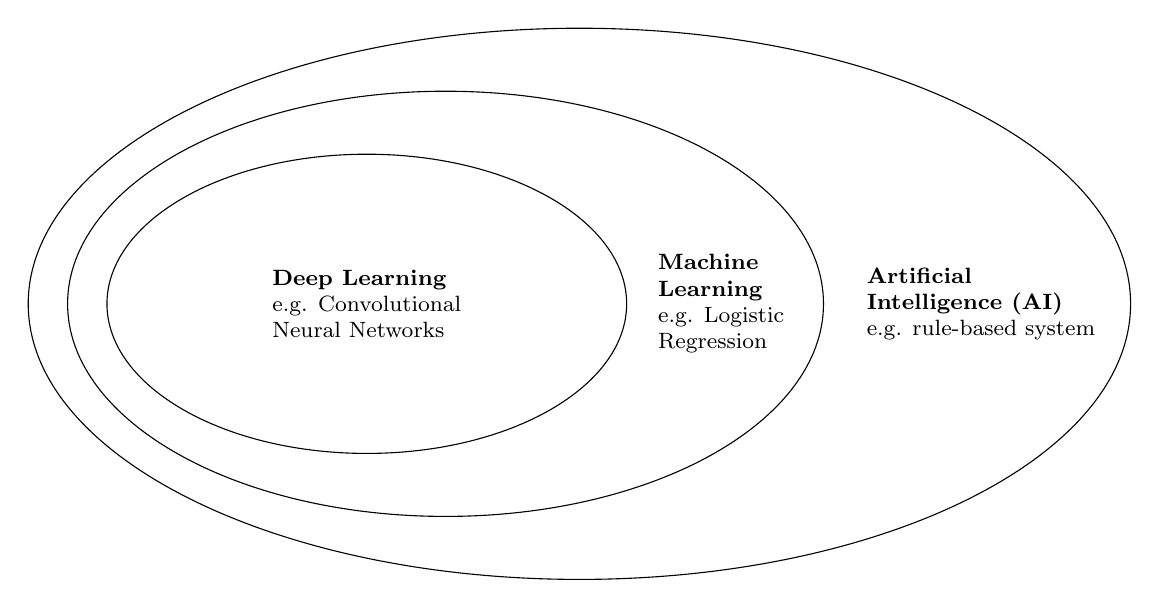
\begin{tikzpicture}[fill=white, font=\footnotesize]
            \draw (0, 0) ellipse (7.0 and 3.5);
            \node[align=left] at (5.1, 0.0) {\textbf{Artificial}\\ \textbf{Intelligence (AI)}\\e.g. rule-based system};
            
            \draw (-1.7, 0) ellipse (4.8 and 2.7) (1.8, 0.0) node[align=left] {\textbf{Machine}\\ \textbf{Learning}\\ e.g. Logistic\\ Regression};
            
            \draw (-2.7, 0) ellipse (3.3 and 1.9) (-2.7, 0.0) node[align=left] {\textbf{Deep Learning}\\ e.g. Convolutional\\ Neural Networks};
        \end{tikzpicture}
    \end{figure}
\end{frame}

\begin{frame}
\frametitle{Why now?}
    \begin{itemize}
        \item \textbf{Technology revolution}---vector processors (e.g. GPGPUs), auto-gradient software
        \item \textbf{Data availability}---large, partially freely available, collections of labeled data
        \item \textbf{Mathematical advances}---latest addition, investigation of new model elements, e.g. activation functions, normalization
    \end{itemize}
\end{frame}

\begin{frame}
\frametitle{Learning Approaches}
    \begin{itemize}
        \item \textbf{Supervised learning:} Learn by ``mimicking supervisor'', i.e. pattern annotations\\ 
        examples: image classification, stock forecasting
        \item \textbf{Unsupervised learning:} Determine patterns purely based on data\\ examples: customer cluster analysis, distribution estimation
        \item \textbf{Reinforcement learning:} Pavlov-style learning with punishment and reward in dynamic environments\\
        examples: game AIs, e.g. AlphaGo or Dota OpenAI
    \end{itemize}
\end{frame}

\begin{frame}
\frametitle{Terminology}
\begin{columns}
\begin{column}{0.48\textwidth}
    \begin{itemize}
        \item \textbf{Samples} or instances,\\ 
        individual observations in your data,\\
        e.g. an image, a specimen
        \item \textbf{Features} or attributes,\\ 
        single characteristic of a sample,\\
        e.g. a pixel, measured weight
        \item \textbf{Channels} or time,\\
        depth information,\\
        color channels, change over time
    \end{itemize}
\end{column}
\begin{column}{0.48\textwidth}
    \begin{figure}
        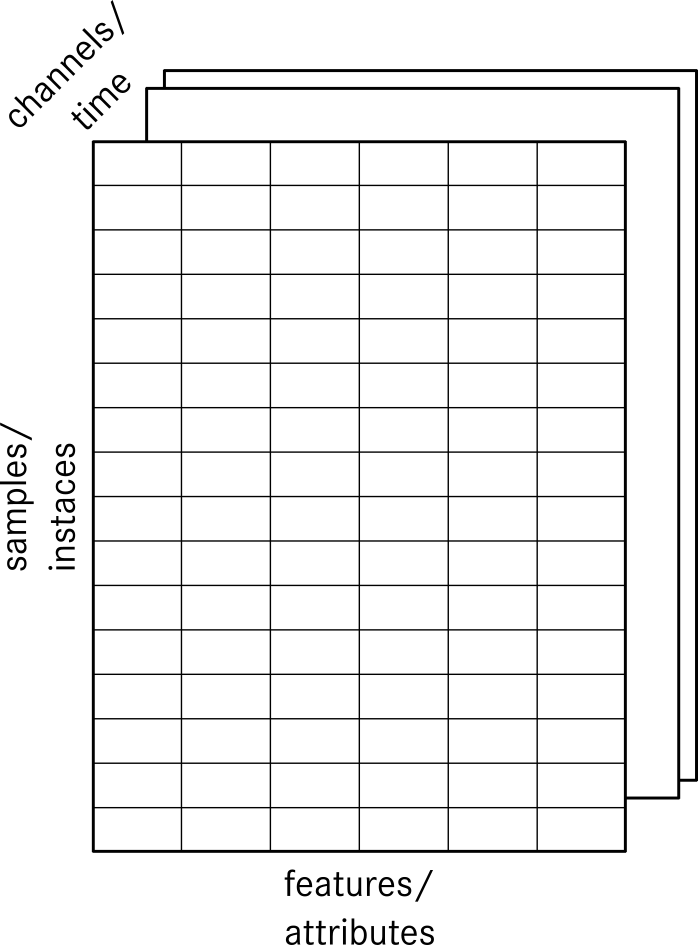
\includegraphics{terminology.png}
    \end{figure}
\end{column}
\end{columns}
\end{frame}

\begin{frame}
\frametitle{MNIST Dataset}

\begin{itemize}
\item \textbf{Goal for today:} classification of handwritten digits
\item 70000 images, each $28\times 28$ pixels, gray-scale
\end{itemize}

\begin{figure}
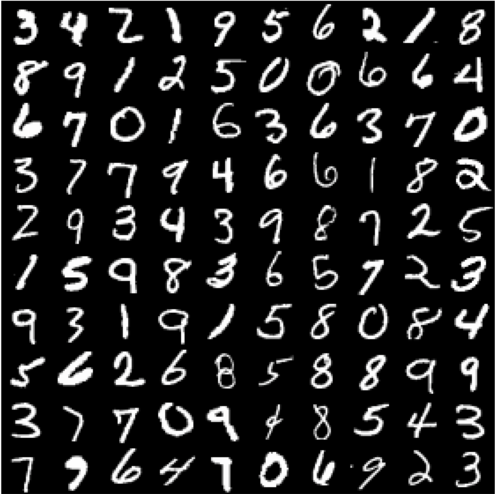
\includegraphics[height=0.6\textheight]{mnist.png}
\end{figure}
\end{frame}

\begin{frame}
\frametitle{Notation Disclaimer}
\begin{itemize}
    \item \textbf{Small letters:} vectors or matrices, e.g. $x$ or $y$
    \item \textbf{Hats:} predictions or estimates, e.g. $\hat{y}$
    \item \textbf{Indices:} elements of vectors and matrices, e.g. $x_{i}$
\end{itemize}

\medskip
\end{frame}

\begin{frame}
\frametitle{Linear Regression}
    \begin{columns}
        \begin{column}{0.43\textwidth}
            \begin{figure}
                \begin{tikzpicture}
                    \begin{axis}[
                        width=\linewidth, 
                        grid=both,
                        grid style={line width=.3pt, draw=presentblue!10},
                        major grid style={line width=.3pt, draw=presentblue!10},
                        minor tick num=3,
                        xlabel={$x$},
                        ylabel={$y$}, 
                        ticks=none,
                        axis x line=center,
                        axis y line=center,
                        xmin=-0.1,
                        xmax=3.0,
                        ymin=-0.1,
                        ymax=1.6
                    ]
                    \only<1->{\addplot [presentblue, only marks, mark size=1pt] coordinates {
                        (0.3, 0.10054215032765762)
                        (0.4263157894736842, 0.12363160260273953)
                        (0.5526315789473685, 0.2228985962683488)
                        (0.6789473684210527, 0.32110283680834006)
                        (0.8052631578947369, 0.3464254484709207)
                        (0.9315789473684213, 0.530973472751518)
                        (1.0578947368421054, 0.508700039361571)
                        (1.1842105263157896, 0.5115642913251457)
                        (1.310526315789474, 0.6517708510332498)
                        (1.4368421052631581, 0.7372626388813315)
                        (1.5631578947368425, 0.7555802030144961)
                        (1.6894736842105267, 0.8020873099226213)
                        (1.8157894736842108, 0.920859494738636)
                        (1.9421052631578952, 0.9025123937365214)
                        (2.0684210526315794, 1.0124087289206862)
                        (2.1947368421052635, 1.081906810760111)
                        (2.3210526315789477, 1.089021024213448)
                        (2.447368421052632, 1.3056222105270976)
                        (2.573684210526316, 1.2573605236570795)
                        (2.7, 1.2546989788028189)
                    };}
                    \node<1-> at (axis cs:1.8,0.5) [presentblue] {\footnotesize\emph{data}};
                    
                    \only<2->{\addplot [presentred, thick, mark=none] {0.5*x};}
                    \node<2-> at (axis cs:2.0,1.3) [presentred] {\footnotesize\emph{model}};
                    \end{axis} 
                \end{tikzpicture}
            \end{figure}
        \end{column}
        \begin{column}{0.53\textwidth}
            \begin{itemize}
                \item<1-> \textbf{Data set:} $\{samples, labels\}=\{x, y\}$
                \item<2-> \textbf{Model:} definition $\hat{y}=wx+b$\\ with $w$ and $b$ trainable parameters
                \item<3-> \textbf{Loss function:} or cost/objective\\
                $J(w,b)=MSE(w,b)=\frac{1}{N}\sum_{i=1}^{N}(y_i-\hat{y_i})^2$
                \item<4-> \textbf{Train:} the model, e.g. optimization\\
                $\hat{w}, \hat{b}=\argmin J(w, b)$ \\
                
            \end{itemize}
        \end{column}
    \end{columns}

    \bigskip
    \begin{itemize}
        \item<5>
            \begin{center}
                \textbf{Basic recipe for most machine learning algorithms}
            \end{center}
    \end{itemize}
\end{frame}

\begin{frame}
\frametitle{Optimization: Gradient Descent}

\begin{itemize}
    \item Iterative optimization technique, weight update in direction of negative gradient
\end{itemize}
\begin{center}$w_{i+1}=w_{i}-lr\nabla_{w_{i}}J(w_i)$\end{center}
\vspace{-0.7cm}
\begin{columns}
    \begin{column}{0.48\textwidth}
        \begin{figure}
            \begin{tikzpicture}
            \begin{axis}[
                width=\linewidth,
                height=0.6\textheight, 
                grid=both,
                grid style={line width=.3pt, draw=presentblue!10},
                major grid style={line width=.3pt, draw=presentblue!10},
                minor tick num=3,
                xlabel={$x$},
                ylabel={$y$}, 
                ticks=none,
                axis x line=center,
                axis y line=center,
                xmin=-0.1,
                xmax=3.0,
                ymin=-0.1,
                ymax=1.6
            ]
            
            \addplot [presentred, thick, mark=none, dashed, domain=0:4] {0.1*(x - 1.5) + 0.75};
            \node at (axis cs:0.3,0.7) [presentred] {\footnotesize$w_{1}$};
            \addplot [presentred, thick, mark=none, dashed, domain=0:4] {0.25*(x - 1.5) + 0.75)};
            \node at (axis cs:0.3,0.35) [presentred] {\footnotesize$w_{2}$};
            \addplot [presentred, thick, mark=none] {0.5*x};
            \node at (axis cs:2.2,1.3) [presentred] {\footnotesize$w_{s}$};
            
            
            \addplot [presentblue, only marks, mark size=1pt] coordinates {
                (0.3, 0.10054215032765762)
                (0.4263157894736842, 0.12363160260273953)
                (0.5526315789473685, 0.2228985962683488)
                (0.6789473684210527, 0.32110283680834006)
                (0.8052631578947369, 0.3464254484709207)
                (0.9315789473684213, 0.530973472751518)
                (1.0578947368421054, 0.508700039361571)
                (1.1842105263157896, 0.5115642913251457)
                (1.310526315789474, 0.6517708510332498)
                (1.4368421052631581, 0.7372626388813315)
                (1.5631578947368425, 0.7555802030144961)
                (1.6894736842105267, 0.8020873099226213)
                (1.8157894736842108, 0.920859494738636)
                (1.9421052631578952, 0.9025123937365214)
                (2.0684210526315794, 1.0124087289206862)
                (2.1947368421052635, 1.081906810760111)
                (2.3210526315789477, 1.089021024213448)
                (2.447368421052632, 1.3056222105270976)
                (2.573684210526316, 1.2573605236570795)
                (2.7, 1.2546989788028189)
            };
            \node at (axis cs:1.8,0.5) [presentblue] {\footnotesize\emph{data}};
            \end{axis} 
            \end{tikzpicture}
        \end{figure}
    \end{column}
    \begin{column}{0.48\textwidth}
        \begin{figure}
            
\begin{tikzpicture}
            \begin{axis}[
            width=\linewidth, 
            height=0.6\textheight, 
            grid=both,
            grid style={line width=.3pt, draw=presentblue!10},
            major grid style={line width=.3pt, draw=presentblue!10},
            minor tick num=3,
            xlabel={$w$},
            ylabel={$J$}, 
            ticks=none,
            axis x line=center,
            axis y line=center,
            xmin=-0.1,
            xmax=3.0,
            ymin=-0.1,
            ymax=1.6
            ]
            % domain=0.25:2.75
            \addplot [black, thick, mark=none, smooth, samples=50, domain=0.3:2.7] {0.9*(x-1.5)^2 + 0.2};
            \addplot [presentred, only marks, mark size=2pt] coordinates {
                (1.5, 0.2)
                (1.0, 0.425)
                (0.5, 1.1)
            };
            \addplot [presentred, mark=none] coordinates {
                (1.5, 0.05)
                (1.5, 0.15)
            };
            \addplot [presentred, mark=none] coordinates {
                (1.0, 0.05)
                (1.0, 0.37)
            };
            \addplot [presentred, mark=none] coordinates {
                (0.5, 0.05)
                (0.5, 1.00)
            };
            \addplot [presentblue, mark=none] coordinates {
                (0.53, 0.95)
                (0.53, 0.43)
                (0.93, 0.43)
            };
            \draw [->, presentred](axis cs:0.57,1.07)--(axis cs:0.98,0.48);
            \node at (axis cs:1.20,0.8) [presentblue] {$lr\frac{dJ}{dw}$};
            \node at (axis cs:0.7,0.1) [presentred] {\footnotesize$w_{1}$};
            \node at (axis cs:1.2,0.1) [presentred] {\footnotesize$w_{2}$};
            \node at (axis cs:1.7,0.1) [presentred] {\footnotesize$w_{s}$};
            \end{axis} 
            \end{tikzpicture}
        \end{figure}
    \end{column}
\end{columns}
\begin{itemize}
    \item $lr$ is learning rate, gradient update factor
    \item \textbf{Stochastic gradient descent (SGD)}, sample subset (\textbf{batch}) updates
\end{itemize}
\end{frame}

\begin{frame}
\frametitle{Bias Trick}

\begin{itemize}
\item Cumbersome to keep track of weights $w$ and bias $b$
\item \textbf{Idea:} fuse both into single weight matrix

\begin{alignat*}{11}
\hat{y}&=&w&x&+b&\leftrightarrow&\hat{y}&=&w&x \\
\hat{y}&=&\begin{pmatrix}
w_{1} \\
w_{2} \\
\vdots \\
w_{n}
\end{pmatrix}'&
\begin{pmatrix}
x_{i,1}\\
x_{i,2}\\
\vdots\\
x_{i,n}\\
\end{pmatrix}&+b&\leftrightarrow&\hat{y}&=&
\begin{pmatrix}
\textbf{b} \\
w_{1} \\
w_{2} \\
\vdots \\
w_{n}
\end{pmatrix}'&
\begin{pmatrix}
\textbf{1}\\
x_{i,1}\\
x_{i,2}\\
\vdots\\
x_{i,n}\\
\end{pmatrix}
\end{alignat*}
\end{itemize}
\end{frame}

\subsection{Logistic Regression}
\label{subsec:logistic-regression}

\begin{frame}
\frametitle{Pattern Recognition Types}
    \begin{columns}
        \begin{column}{0.48\textwidth}
            \begin{itemize}
                \item \textbf{Regression:} predict continuous value, e.g. stock price, $y\in\mathbb{R}$
                \item \textbf{Classification:} assign sample to a category, e.g. ``spam''/``no spam''\\special form of regression,\\ where $y$ in fixed interval
            \end{itemize}
        \end{column}
        \begin{column}{0.48\textwidth}
            \begin{figure}
                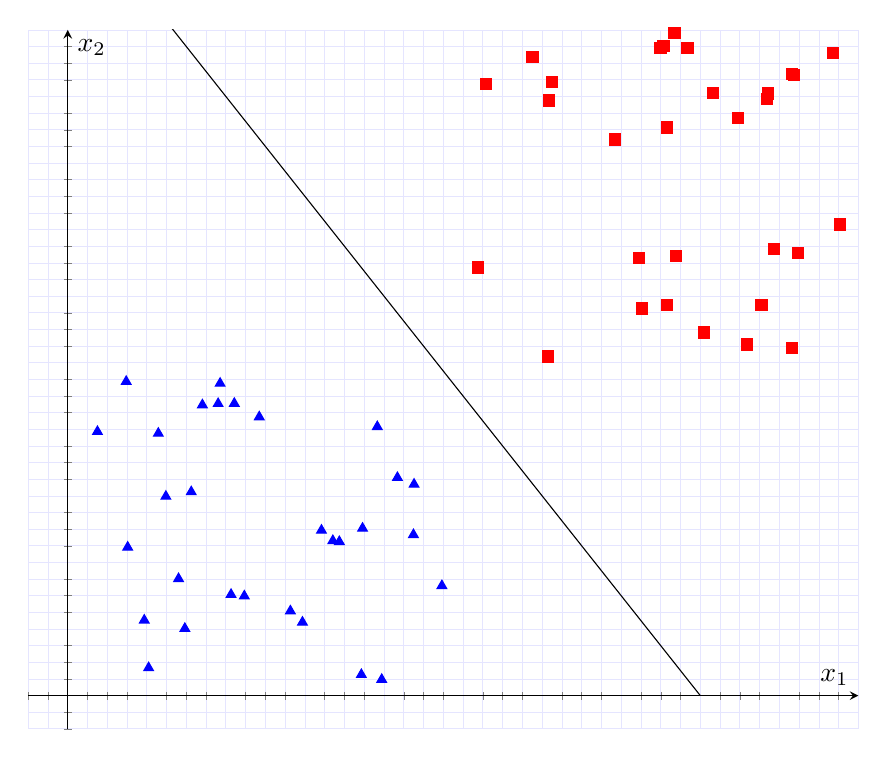
\begin{tikzpicture}
                \begin{axis}[
                    width=\linewidth, 
                    grid=both,
                    grid style={line width=.3pt, draw=presentblue!10},
                    major grid style={line width=.3pt, draw=presentblue!10},
                    minor tick num=3,
                    xlabel={$x_1$},
                    ylabel={$x_2$}, 
                    ticks=none,
                    axis x line=center,
                    axis y line=center,
                    xmin=-0.1,
                    xmax=2.0,
                    ymin=-0.1,
                    ymax=2.0
                ]
                \addplot [presentblue, only marks, mark size=2pt, mark=triangle*] coordinates {
                    (0.3405210822112612, 0.8733467370280228)
                    (0.6417180817230281, 0.4966306166288442)
                    (0.31236861944953176, 0.6121119482760103)
                    (0.4843845705001969, 0.8372723451578254)
                    (0.6705319198897809, 0.46544265493212356)
                    (0.15159623290041857, 0.44576239992026545)
                    (0.9463452893119627, 0.33010610736211987)
                    (0.19348743132666624, 0.22660283230073164)
                    (0.2961562717918107, 0.20157698331379592)
                    (0.38534371092248065, 0.9381135102799997)
                    (0.0750871559631675, 0.7932733927855736)
                    (0.14786222142469718, 0.9437344260840296)
                    (0.5936565086474459, 0.22034859139209484)
                    (0.22907523223663817, 0.7878697366360873)
                    (0.794139162809545, 0.048334139863450254)
                    (0.2481683008839609, 0.5986112990477678)
                    (0.28024639511041294, 0.35123819610592255)
                    (0.7426502500585584, 0.06302390692215687)
                    (0.4465644429635456, 0.29914396434886015)
                    (0.7829307093180131, 0.8078686578775368)
                    (0.38036767570222685, 0.8771510877252888)
                    (0.5630903124576907, 0.2542147707582497)
                    (0.8338634277199973, 0.6550543205600249)
                    (0.8759184599366046, 0.6349455271372683)
                    (0.6869371856928128, 0.46250259195124)
                    (0.4212924892722074, 0.8777507521988864)
                    (0.874384938038331, 0.4834185999120415)
                    (0.2045721844969517, 0.0834946363978849)
                    (0.41302308334280347, 0.30372338532728305)
                    (0.7456467692023212, 0.5026216907475388)
                };
                \addplot [presentred, only marks, mark size=2pt, mark=square*] coordinates {
                    (1.7706837759950487, 1.808884456339976)
                    (1.6097673166601565, 1.0910700963071096)
                    (1.8311427531366666, 1.043397970524071)
                    (1.7686274677101825, 1.7929387383883477)
                    (1.8476473528536392, 1.3287310154974328)
                    (1.51561309479197, 1.7071106254688428)
                    (1.4441136349948995, 1.3151875726875542)
                    (1.6320240433560618, 1.8106133358232555)
                    (1.93615150297599, 1.9318761344130344)
                    (1.6957150249499564, 1.7353082711966865)
                    (1.3832499009666868, 1.6706984272443974)
                    (1.5390778241411607, 1.3212483573991296)
                    (1.5067423770579214, 1.951642819491536)
                    (1.5162449533753577, 1.1744133372978611)
                    (1.452290644909902, 1.1628763191277276)
                    (1.215300195996602, 1.0190784373594854)
                    (1.832559930658315, 1.8667682767915506)
                    (1.7174600650559508, 1.0548065370692519)
                    (1.2178766103535255, 1.7877897361036623)
                    (1.5675863098843703, 1.946616980060258)
                    (1.9539865940177632, 1.415630588037017)
                    (1.0386711055996827, 1.28647932022736)
                    (1.4994662399845793, 1.9459071761746531)
                    (1.057157101434958, 1.8380166331031762)
                    (1.7853872352436764, 1.3426683001589166)
                    (1.75459402308149, 1.1746356610150874)
                    (1.534515821721585, 1.990233613715762)
                    (1.8364540007603098, 1.863869583052054)
                    (1.2251698093011876, 1.8446796325215797)
                    (1.1756480589317504, 1.9193842816924964)
                };
                \addplot [black, mark=none, domain=0:1.6] {-1.5*x+2.4};
                \end{axis}
                \end{tikzpicture}
            \end{figure}
        \end{column}
    \end{columns}
\end{frame}

\begin{frame}
\frametitle{Logistic Regression}

\begin{columns}
    \begin{column}{0.48\textwidth}
        \begin{figure}
            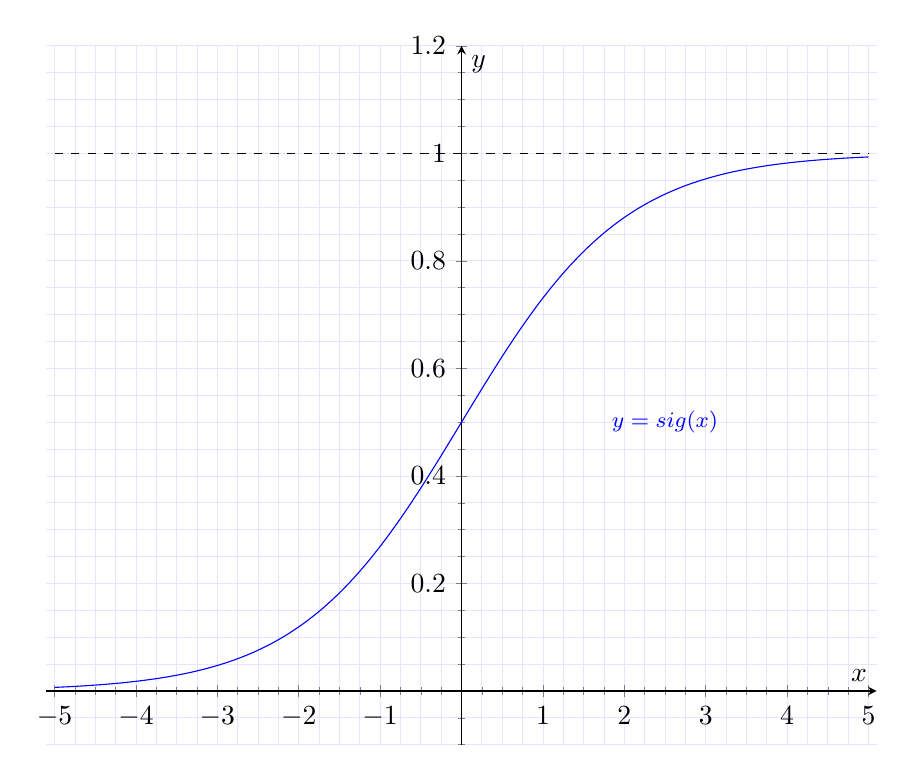
\begin{tikzpicture}
            \begin{axis}[
                width=\linewidth, 
                grid=both,
                grid style={line width=.3pt, draw=presentblue!10},
                major grid style={line width=.3pt, draw=presentblue!10},
                minor tick num=3,
                xlabel={$x$},
                ylabel={$y$}, 
                axis x line=center,
                axis y line=center,
                xmin=-5.1,
                xmax=5.1,
                ymin=-0.1,
                ymax=1.2
            ]
            \addplot [presentblue, mark=none, smooth, samples=50] {1/(1 + e^-x)};
            \addplot [black, dashed, mark=none] {1};
            \node at (axis cs:2.5,0.5) [presentblue] {\footnotesize$y=sig(x)$};
            \end{axis}
            \end{tikzpicture}
        \end{figure}
    \end{column}
    \begin{column}{0.48\textwidth}
        \begin{itemize}
            \item Squash linear regression output into fixed interval, e.g. $y\in[0,1]$
            \item Interpretation: \textbf{probability} of sample belonging to a binary class
            \item \textbf{sigmoid-/logistic} function: $sig(z)=\frac{1}{1+e^{-x}}$
            \item \textbf{Model:} $h=sig(wx)=\frac{1}{1+e^{-wx}}$
            \item \textbf{Prediction:} $\hat{y}=1$ if $h\geq 0.5$\\\hspace{2.15cm}$\hat{y}=0$ if $h<0.5$
        \end{itemize}
    \end{column}
\end{columns}
\end{frame}

\begin{frame}
\frametitle{Logistic Regression}
\begin{columns}
    \begin{column}{0.48\textwidth}
        \begin{itemize}
            \item \textbf{Data set} must be mapped
            \begin{itemize}
                \item \tikz{\node[fill=presentred, rectangle ,minimum width=0.2cm,minimum height=0.2cm,inner sep=0pt] at (0,0) {};} $\rightarrow 0$
                \item \tikz{\node[fill=presentblue, isosceles triangle,isosceles triangle stretches,shape border rotate=90,minimum width=0.2cm,minimum height=0.2cm,inner sep=0pt] at (0,0) {};} $\rightarrow 1$
            \end{itemize}
            \item \textbf{Model:} $h=sig(wx)=\frac{1}{1+e^{-wx}}$
            \item \textbf{Loss function:} $J(w)=MSE(w)=\frac{1}{n}\sum_{i=1}^{n}(y-\hat{y})^2$\\
            \medskip
            $\frac{dJ}{dw}=(\hat{y}-y)*(\hat{y}-\hat{y}^2)*x$
            \item \textbf{Train:} gradient descent optimization
        \end{itemize}
    \end{column}
    \begin{column}{0.48\textwidth}
        \begin{figure}
            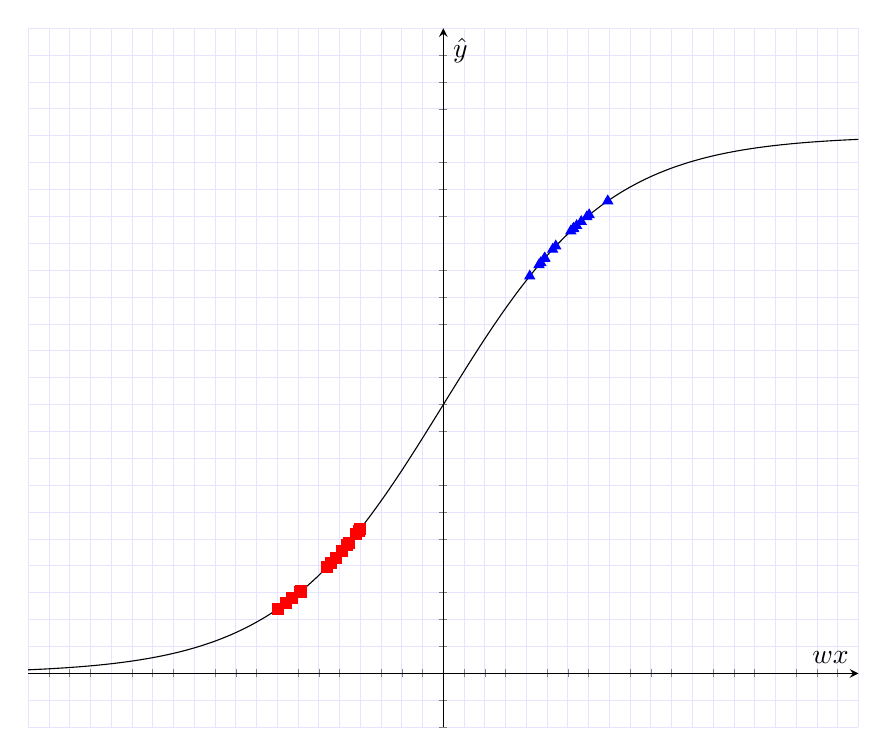
\begin{tikzpicture}
            \begin{axis}[
                width=\linewidth, 
                grid=both,
                grid style={line width=.3pt, draw=presentblue!10},
                major grid style={line width=.3pt, draw=presentblue!10},
                minor tick num=3,
                xlabel={$wx$},
                ylabel={$\hat{y}$}, 
                ticks=none,
                axis x line=center,
                axis y line=center,
                xmin=-5.0,
                xmax=5.0,
                ymin=-0.1,
                ymax=1.2
            ]
            \addplot [presentblue, only marks, mark size=2pt, mark=triangle*] coordinates {
                (1.6611027206330746, 0.8403859746482719)
                (1.7284679911037832, 0.8492163546084681)
                (1.980447929430528, 0.8787289035454036)
                (1.354218630150888, 0.7948184668511403)
                (1.6057278678332159, 0.8328174119222866)
                (1.1740038141330658, 0.7638679613026638)
                (1.5654305489944456, 0.8271312208936279)
                (1.0406374778006744, 0.7389729891261709)
                (1.2175306663046495, 0.7716287006468228)
                (1.15212482162792, 0.7598988102612867)
                (1.222433948485342, 0.7724915954912219)
                (1.3168137689858914, 0.7886511122722238)
                (1.5356204800918496, 0.822827169753855)
                (1.5691829504301005, 0.8276671001940339)
                (1.7567986844605772, 0.8528082645120062)
            };
            \addplot [presentred, only marks, mark size=2pt, mark=square*] coordinates {
                (-1.0196347184444567, 0.2650985590592027)
                (-1.0022522286115616, 0.26849883685519904)
                (-1.1557365565390303, 0.23944283798422109)
                (-1.3974671254713573, 0.1982183480307425)
                (-1.1606958459299377, 0.2385408693182452)
                (-1.715658735359114, 0.15243119145146328)
                (-1.8951996922132972, 0.13065273979168898)
                (-1.7293798235626427, 0.15066692430088222)
                (-1.2251200041104404, 0.2270366802689441)
                (-1.2937274869746527, 0.21522256323939018)
                (-1.3545206550890927, 0.2051322826820219)
                (-1.8193666281874563, 0.13950988991290472)
                (-1.1391575506830613, 0.2424750692801325)
                (-1.9905389939009734, 0.12019985119782262)
                (-1.0480273799098105, 0.2596040778945661)
                
            };
        
            \addplot [black, mark=none, smooth, samples=50] {1/(1 + e^-x)};
            \end{axis}
            \end{tikzpicture}
        \end{figure}
    \end{column}
\end{columns}
\end{frame}

\subsection{Libraries}
\label{subsec:libraries}

\begin{frame}
\frametitle{Autograd Frameworks: TensorFlow \& Co}

\begin{columns}
    \begin{column}{0.48\textwidth}
        \begin{itemize}
            \item \textbf{Numerical} and \textbf{autograd} libraries
            \item \textbf{Eager} and \textbf{flow graph} computation
            \item Multiple supported devices\\
            \textbf{CPU, GPU}, TPU, smartphone
            \item TensorFlow (Google), MXNet (Amazon), PyTorch (Facebook)
            \item \textbf{Keras}---neural network wrapper for\\
            TensorFlow and MXNet backends
        \end{itemize}
    \end{column}
    \begin{column}{0.23\textwidth}
        \begin{figure}
            \centering
            
\includegraphics[height=0.6\linewidth]{tensorflow.png}
            \imageright{Google}
        \end{figure}
        \vfill
        \begin{figure}
            \centering
            
\includegraphics[width=0.9\linewidth]{mxnet.png}
            \imageright{Apache}
        \end{figure}
    \end{column}
    \begin{column}{0.23\textwidth}
        \vspace{2.5cm}
        \begin{figure}
            \centering
            
\includegraphics[width=0.9\linewidth]{pytorch.png}
            \imageright{PyTorch}
        \end{figure}
        \begin{figure}
            \centering
            
\includegraphics[width=0.9\linewidth]{keras.png}
            \imageright{Keras}
            \vspace{1.2cm}
        \end{figure}
    \end{column}
\end{columns}
\end{frame}

\begin{frame}[fragile]
\frametitle{Keras an Example}

\begin{lstlisting}[language=Python]
from keras.models import Sequential
from keras.layers import Dense

# Logistic regression model with two features
model = Sequential()
model.add(Dense(1, input_dim=2, activation="sigmoid"))

# Model compilation
model.compile(loss="mse", optimizer="sgd")

# Fit the model, i.e. optimize J for 10 iterations
model.fit(x, y, epochs=10)
\end{lstlisting}

\end{frame}

\subsection{Exercise: Logistic Regression}
\label{subsec:exercise-logistic-regression}

\begin{frame}
\frametitle{Exercise 1: Warm-up}

\begin{figure}
    \centering
    \begin{tikzpicture}[]
    \node [inner sep=0pt,above right] { %
        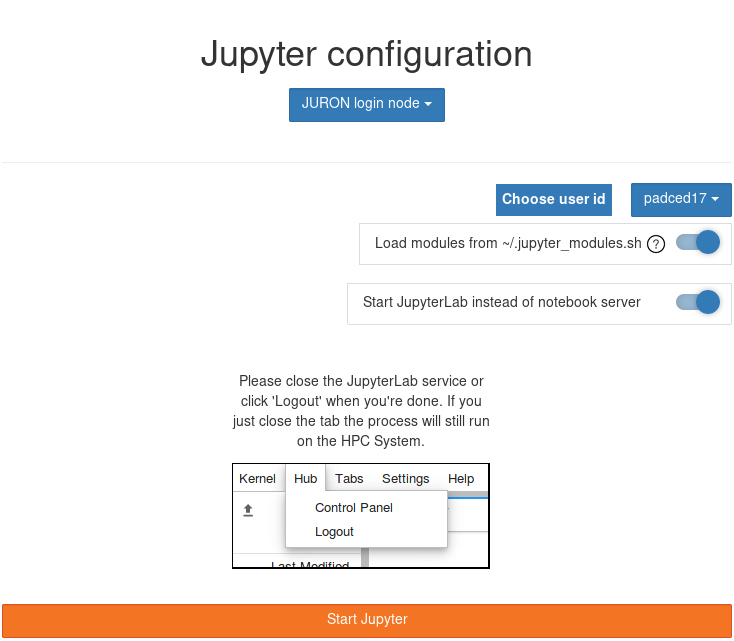
\includegraphics[width=0.5\linewidth]{jupyter.png} %
    };
    % show origin
    \draw [line width=0.6mm, presentred] (7.05, 4.05) ellipse (0.5 and 0.25);
    \end{tikzpicture}
\end{figure}

\end{frame}

\begin{frame}
\frametitle{Exercise: Logistic Regression}

\begin{columns}
    \begin{column}{0.48\textwidth}
        \begin{itemize}
            \item \textbf{Data set} must be mapped
            \begin{itemize}
                \item \tikz{\node[fill=presentred, rectangle ,minimum width=0.2cm,minimum height=0.2cm,inner sep=0pt] at (0,0) {};} $\rightarrow 0$
                \item \tikz{\node[fill=presentblue, isosceles triangle,isosceles triangle stretches,shape border rotate=90,minimum width=0.2cm,minimum height=0.2cm,inner sep=0pt] at (0,0) {};} $\rightarrow 1$
            \end{itemize}
            \item \textbf{Model:} $h=sig(wx)=\frac{1}{1+e^{-wx}}$
            \item \textbf{Loss function:} $J(w)=MSE(w)=(y-\hat{y})^2$\\
            \medskip
            $\frac{dJ}{dw}=(\hat{y}-y)*(\hat{y}-\hat{y}^2)*x$
            \item \textbf{Train:} $w_{i+1}=w_{i}-lr\frac{dJ}{dw_i}$
            \item \href{https://jupyter-jsc.fz-juelich.de/}{https://jupyter-jsc.fz-juelich.de/}
        \end{itemize}
    \end{column}
    \begin{column}{0.48\textwidth}
        \begin{figure}
            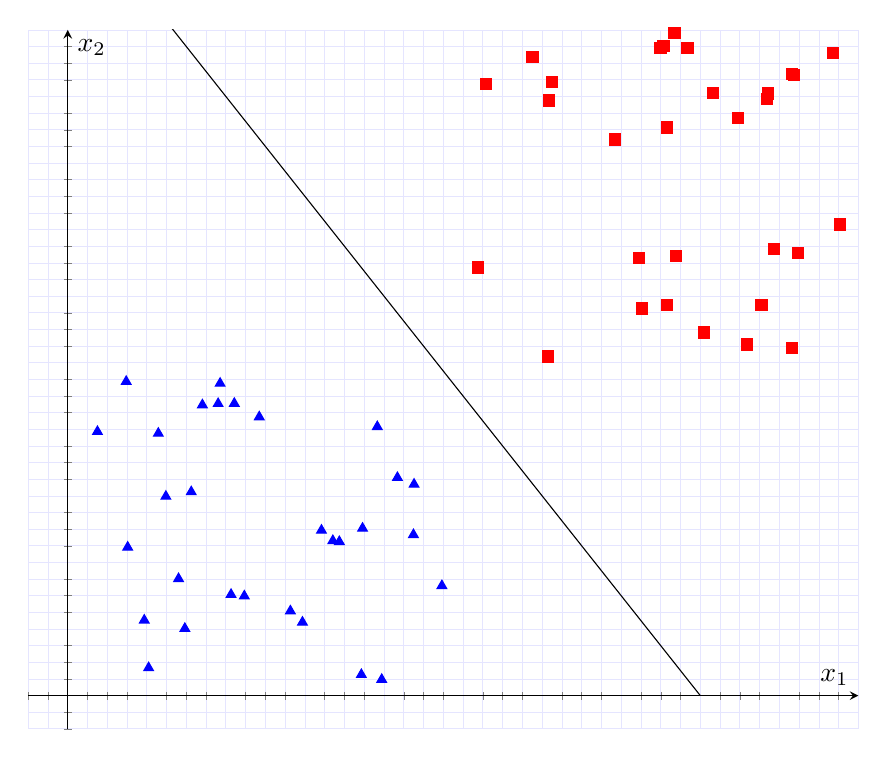
\begin{tikzpicture}
            \begin{axis}[
            width=\linewidth, 
            grid=both,
            grid style={line width=.3pt, draw=presentblue!10},
            major grid style={line width=.3pt, draw=presentblue!10},
            minor tick num=3,
            xlabel={$x_1$},
            ylabel={$x_2$}, 
            ticks=none,
            axis x line=center,
            axis y line=center,
            xmin=-0.1,
            xmax=2.0,
            ymin=-0.1,
            ymax=2.0
            ]
            \addplot [presentblue, only marks, mark size=2pt, mark=triangle*] coordinates {
                (0.3405210822112612, 0.8733467370280228)
                (0.6417180817230281, 0.4966306166288442)
                (0.31236861944953176, 0.6121119482760103)
                (0.4843845705001969, 0.8372723451578254)
                (0.6705319198897809, 0.46544265493212356)
                (0.15159623290041857, 0.44576239992026545)
                (0.9463452893119627, 0.33010610736211987)
                (0.19348743132666624, 0.22660283230073164)
                (0.2961562717918107, 0.20157698331379592)
                (0.38534371092248065, 0.9381135102799997)
                (0.0750871559631675, 0.7932733927855736)
                (0.14786222142469718, 0.9437344260840296)
                (0.5936565086474459, 0.22034859139209484)
                (0.22907523223663817, 0.7878697366360873)
                (0.794139162809545, 0.048334139863450254)
                (0.2481683008839609, 0.5986112990477678)
                (0.28024639511041294, 0.35123819610592255)
                (0.7426502500585584, 0.06302390692215687)
                (0.4465644429635456, 0.29914396434886015)
                (0.7829307093180131, 0.8078686578775368)
                (0.38036767570222685, 0.8771510877252888)
                (0.5630903124576907, 0.2542147707582497)
                (0.8338634277199973, 0.6550543205600249)
                (0.8759184599366046, 0.6349455271372683)
                (0.6869371856928128, 0.46250259195124)
                (0.4212924892722074, 0.8777507521988864)
                (0.874384938038331, 0.4834185999120415)
                (0.2045721844969517, 0.0834946363978849)
                (0.41302308334280347, 0.30372338532728305)
                (0.7456467692023212, 0.5026216907475388)
            };
            \addplot [presentred, only marks, mark size=2pt, mark=square*] coordinates {
                (1.7706837759950487, 1.808884456339976)
                (1.6097673166601565, 1.0910700963071096)
                (1.8311427531366666, 1.043397970524071)
                (1.7686274677101825, 1.7929387383883477)
                (1.8476473528536392, 1.3287310154974328)
                (1.51561309479197, 1.7071106254688428)
                (1.4441136349948995, 1.3151875726875542)
                (1.6320240433560618, 1.8106133358232555)
                (1.93615150297599, 1.9318761344130344)
                (1.6957150249499564, 1.7353082711966865)
                (1.3832499009666868, 1.6706984272443974)
                (1.5390778241411607, 1.3212483573991296)
                (1.5067423770579214, 1.951642819491536)
                (1.5162449533753577, 1.1744133372978611)
                (1.452290644909902, 1.1628763191277276)
                (1.215300195996602, 1.0190784373594854)
                (1.832559930658315, 1.8667682767915506)
                (1.7174600650559508, 1.0548065370692519)
                (1.2178766103535255, 1.7877897361036623)
                (1.5675863098843703, 1.946616980060258)
                (1.9539865940177632, 1.415630588037017)
                (1.0386711055996827, 1.28647932022736)
                (1.4994662399845793, 1.9459071761746531)
                (1.057157101434958, 1.8380166331031762)
                (1.7853872352436764, 1.3426683001589166)
                (1.75459402308149, 1.1746356610150874)
                (1.534515821721585, 1.990233613715762)
                (1.8364540007603098, 1.863869583052054)
                (1.2251698093011876, 1.8446796325215797)
                (1.1756480589317504, 1.9193842816924964)
            };
            \addplot [black, mark=none, domain=0:1.6] {-1.5*x+2.4};
            \end{axis}
            \end{tikzpicture}
        \end{figure}
    \end{column}
\end{columns}
\end{frame}

\section{Neural Networks}
\label{sec:neural-networks}

\subsection{Motivation}
\label{subsec:motivation}

\begin{frame}
\frametitle{XOR-Problem}
\begin{columns}
    \begin{column}{0.48\textwidth}
        \begin{figure}
            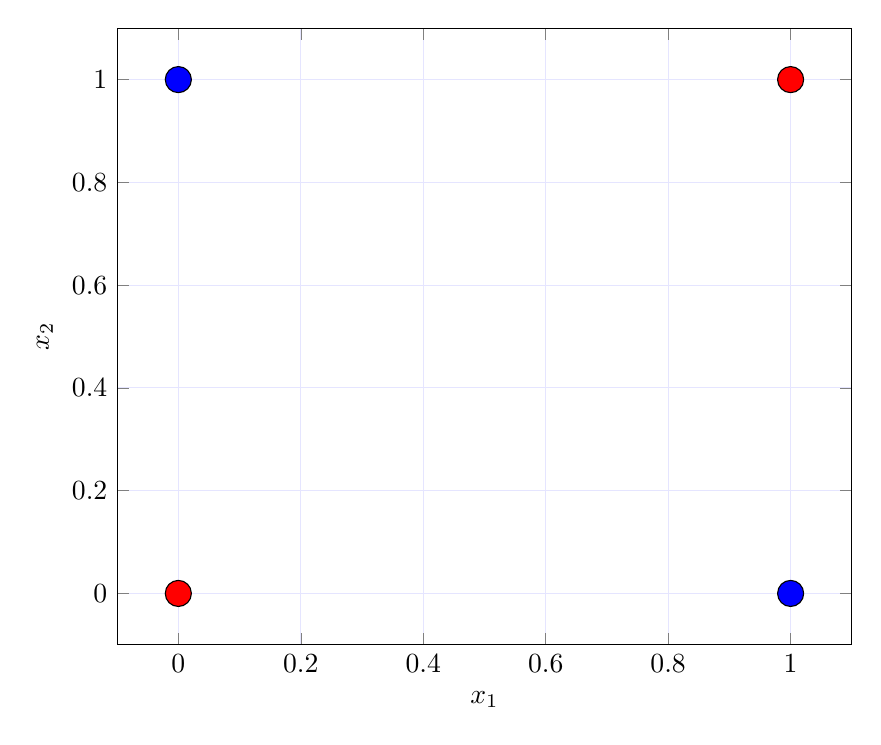
\begin{tikzpicture}
            \begin{axis}[
                width=0.9\linewidth,
                grid=major,
                grid style={line width=.3pt, draw=presentblue!10},
                major grid style={line width=.3pt, draw=presentblue!10},
                %minor tick num=2,
                xlabel={$x_1$},
                ylabel={$x_2$},
                xmin=-0.1,
                xmax=1.1,
                ymin=-0.1,
                ymax=1.1
            ]
            \node[draw, circle, fill=presentred,  radius=0.3cm] at (1, 1) {};
            \node[draw, circle, fill=presentred,  radius=0.3cm] at (0, 0) {};
            \node[draw, circle, fill=presentblue, radius=0.3cm] at (1, 0) {};
            \node[draw, circle, fill=presentblue, radius=0.3cm] at (0, 1) {};
            \end{axis}
            \end{tikzpicture}
        \end{figure}
    \end{column}
    \begin{column}{0.48\textwidth}
        \begin{itemize}
            \item Binary exclusive operator,\\ 
            is $1$ if one operand is $1$, else $0$
            \item Non-linearly separable,\\ 
            logistic regression cannot model problem
            \item \textbf{Idea:} decompose into linear problems
        \end{itemize}
    \end{column}
\end{columns}
\end{frame}

\begin{frame}
\frametitle{XOR-Problem}
\begin{columns}
    \begin{column}{0.32\textwidth}
        \begin{onlyenv}<1->
        \begin{figure}
            \centering
            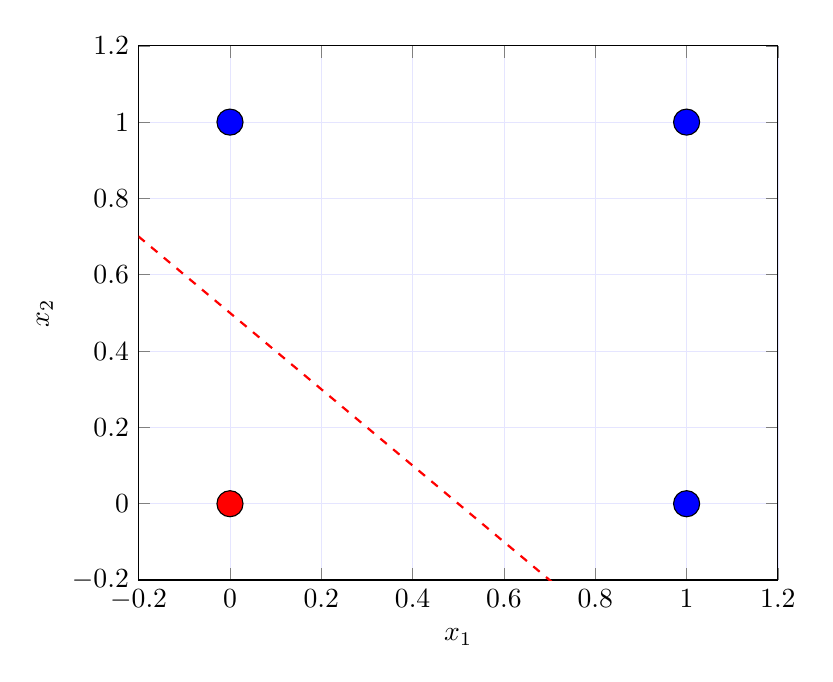
\begin{tikzpicture}
            \begin{axis}[
                width=0.8\linewidth,
                grid=major,
                grid style={line width=.3pt, draw=presentblue!10},
                major grid style={line width=.3pt, draw=presentblue!10},
                xlabel={$x_1$},
                ylabel={$x_2$},
                xmin=-0.2,
                xmax=1.2,
                ymin=-0.2,
                ymax=1.2
            ]
            \node[draw, circle, fill=presentblue, radius=0.05cm] at (1, 1) {};
            \node[draw, circle, fill=presentred,  radius=0.05cm] at (0, 0) {};
            \node[draw, circle, fill=presentblue, radius=0.05cm] at (1, 0) {};
            \node[draw, circle, fill=presentblue, radius=0.05cm] at (0, 1) {};
            \addplot[presentred, thick, dashed, mark=none] {-x + 0.5};
            \end{axis}
            \end{tikzpicture}
        \end{figure}
        \end{onlyenv}
    \end{column}
    \begin{column}{0.32\textwidth}
        \begin{onlyenv}<2->
        \begin{figure}
            \centering
            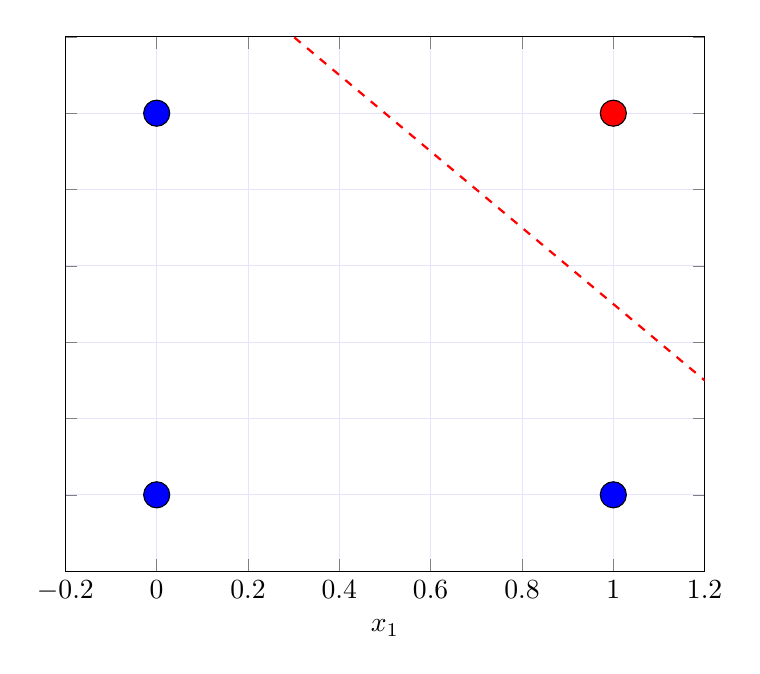
\begin{tikzpicture}
            \begin{axis}[
                width=0.8\linewidth,
                grid=major,
                grid style={line width=.3pt, draw=presentblue!10},
                major grid style={line width=.3pt, draw=presentblue!10},
                xlabel={$x_1$},
                yticklabels={,,},
                xmin=-0.2,
                xmax=1.2,
                ymin=-0.2,
                ymax=1.2,
            ]
            \node[draw, circle, fill=presentred,  radius=0.05cm] at (1, 1) {};
            \node[draw, circle, fill=presentblue, radius=0.05cm] at (0, 0) {};
            \node[draw, circle, fill=presentblue, radius=0.05cm] at (1, 0) {};
            \node[draw, circle, fill=presentblue, radius=0.05cm] at (0, 1) {};
            \addplot[presentred, thick, dashed, mark=none] {-x + 1.5};
            \end{axis}
            \end{tikzpicture}
        \end{figure}
        \end{onlyenv}
    \end{column}
    \begin{column}{0.32\textwidth}
        \begin{onlyenv}<3->
        \begin{figure}
            \centering
            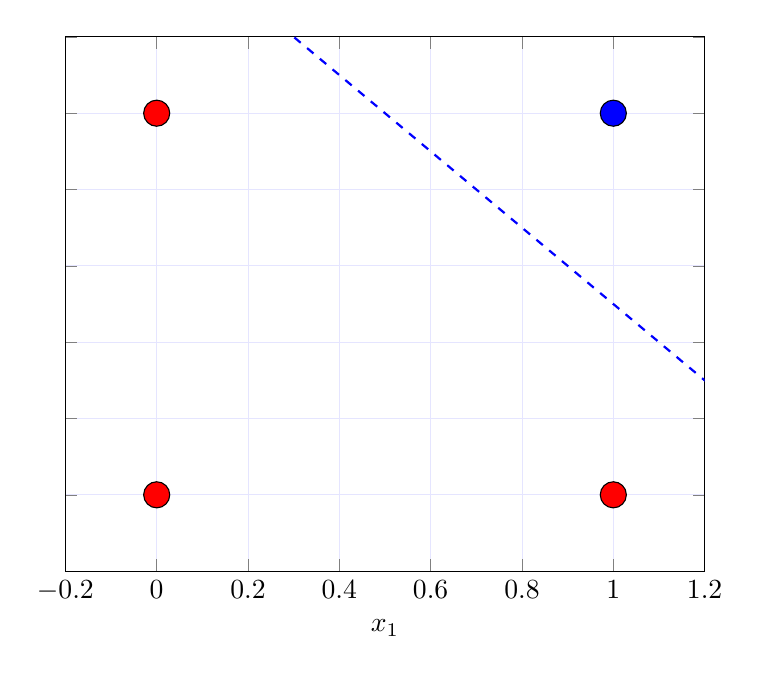
\begin{tikzpicture}
            \begin{axis}[
                width=0.8\linewidth,
                grid=major,
                grid style={line width=.3pt, draw=presentblue!10},
                major grid style={line width=.3pt, draw=presentblue!10},
                xlabel={$x_1$},
                yticklabels={,,},
                xmin=-0.2,
                xmax=1.2,
                ymin=-0.2,
                ymax=1.2,
            ]
            \node[draw, circle, fill=presentblue, radius=0.05cm] at (1, 1) {};
            \node[draw, circle, fill=presentred,  radius=0.05cm] at (0, 0) {};
            \node[draw, circle, fill=presentred,  radius=0.05cm] at (1, 0) {};
            \node[draw, circle, fill=presentred,  radius=0.05cm] at (0, 1) {};
            \addplot[presentblue, thick, dashed, mark=none] {-x + 1.5};
            \end{axis}
            \end{tikzpicture}
        \end{figure}
        \end{onlyenv}
    \end{column}
\end{columns}
\bigskip
\begin{columns}
    \begin{column}{0.32\textwidth}
        \centering
        \begin{onlyenv}<1->
        \textbf{OR-gate}\\
        \medskip
        $h_1=sig(2x_1 + 2x_2 + 1)$
    \end{onlyenv}
    \end{column}
    \begin{column}{0.32\textwidth}
        \centering
        \begin{onlyenv}<2->
        \textbf{NAND-gate}\\
        \medskip
        $h_2=sig(-2x_1 -2x_2 - 1.5)$
    \end{onlyenv}
    \end{column}
    \begin{column}{0.32\textwidth}
        \centering
        \begin{onlyenv}<3->
        \textbf{AND-gate}\\
        \medskip
        $\hat{y}=sig(2h_1 +2h_2 + 3)$
        \end{onlyenv}
    \end{column}
\end{columns}
\end{frame}

\begin{frame}
\frametitle{Fully-connected Neural Network}

\begin{columns}
    \begin{column}{0.48\textwidth}
        \begin{figure}
            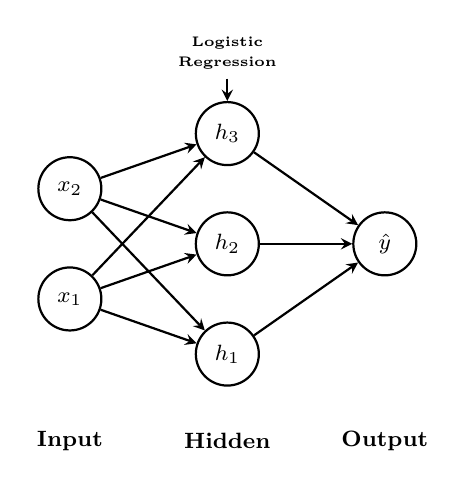
\begin{tikzpicture}
            \node[draw, circle, thick, minimum size=0.8cm] (input1) at (-2,-0.7) {\footnotesize$x_1$};
            \node[draw, circle, thick, minimum size=0.8cm] (input2) at (-2, 0.7) {\footnotesize$x_2$};
            
            \node[draw, circle, thick, minimum size=0.8cm] (hidden1) at (0,-1.4) {\footnotesize$h_1$};
            \node[draw, circle, thick, minimum size=0.8cm] (hidden2) at (0, 0)   {\footnotesize$h_2$};
            \node[draw, circle, thick, minimum size=0.8cm] (hidden3) at (0, 1.4) {\footnotesize$h_3$};
            
            \node[draw, circle, thick, minimum size=0.8cm] (output) at (2, 0) {\footnotesize$\hat{y}$};
            
            \draw[->, >=stealth, thick] (input1)--(hidden1);
            \draw[->, >=stealth, thick] (input1)--(hidden2);
            \draw[->, >=stealth, thick] (input1)--(hidden3);
            
            \draw[->, >=stealth, thick] (input2)--(hidden1);
            \draw[->, >=stealth, thick] (input2)--(hidden2);
            \draw[->, >=stealth, thick] (input2)--(hidden3);
            
            \draw[->, >=stealth, thick] (hidden1)--(output);
            \draw[->, >=stealth, thick] (hidden2)--(output);
            \draw[->, >=stealth, thick] (hidden3)--(output);
            
            \node at (-2, -2.5) {\footnotesize \textbf{Input}};
            \node at ( 0, -2.5) {\footnotesize \textbf{Hidden}};
            \node at ( 2, -2.5) {\footnotesize \textbf{Output}};
            
            \node[align=center] at (0, 2.55) {\textbf{\tiny Logistic}};
            \node[align=center] (reg) at (0, 2.3) {\textbf{\tiny Regression}};
            \draw[->, >=stealth, thick] (reg)--(hidden3);
            \end{tikzpicture}
        \end{figure}
    \end{column}
    \begin{column}{0.48\textwidth}
        \begin{itemize}
            \item Inspired by biological neural network
            \item A \textbf{neuron} is a logistic regression
            \item Neurons are arranged in \textbf{layers}
            \item Layers are \textbf{fully-connected} with subsequent layer, also called \textbf{Dense}
            \item \textbf{Width:} neuron count
            \item \textbf{Depth:} layer count
        \end{itemize}
    \end{column}
\end{columns}
\end{frame}

\subsection{Backpropagation}
\label{subsec:backpropagation}

\begin{frame}
\frametitle{Backpropagation}

\begin{columns}
    \begin{column}{0.48\textwidth}
        \begin{itemize}
            \item Alternate forward and backward pass
            \item \textbf{Hidden layer} are nested functions
            \begin{itemize}
                \item Requires \textbf{chain rule} for gradient
                \item $h'(x)=f'(g(x))*g(x)$
                \item \textbf{Neurons store forward result}
            \end{itemize}
            \item Weight initialization in network\\
            small random numbers
            \item Iterations are now called \textbf{epochs}
        \end{itemize}
    \end{column}
    \begin{column}{0.48\textwidth}
        \begin{figure}
            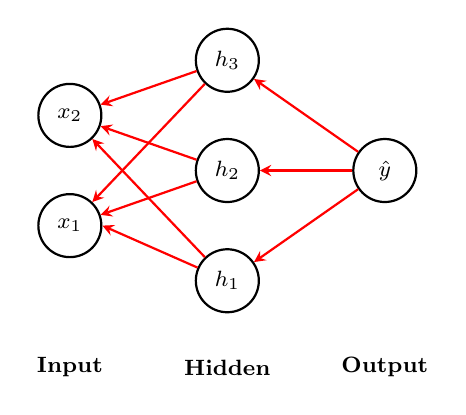
\begin{tikzpicture}
            \node[draw, circle, thick, minimum size=0.8cm] (input1) at (-2,-0.7) {\footnotesize$x_1$};
            \node[draw, circle, thick, minimum size=0.8cm] (input2) at (-2, 0.7) {\footnotesize$x_2$};
            
            \node[draw, circle, thick, minimum size=0.8cm] (hidden1) at (0,-1.4) {\footnotesize$h_1$};
            \node[draw, circle, thick, minimum size=0.8cm] (hidden2) at (0, 0)   {\footnotesize$h_2$};
            \node[draw, circle, thick, minimum size=0.8cm] (hidden3) at (0, 1.4) {\footnotesize$h_3$};
            
            \node[draw, circle, thick, minimum size=0.8cm] (output) at (2, 0) {\footnotesize$\hat{y}$};
            
            \draw[presentred, ->, >=stealth, thick] (hidden1)--(input1.east);
            \draw[presentred, ->, >=stealth, thick] (hidden2)--(input1);
            \draw[presentred, ->, >=stealth, thick] (hidden3)--(input1);
            
            \draw[presentred, ->, >=stealth, thick] (hidden1)--(input2);
            \draw[presentred, ->, >=stealth, thick] (hidden2)--(input2);
            \draw[presentred, ->, >=stealth, thick] (hidden3)--(input2);
            
            \draw[presentred, ->, >=stealth, thick] (output)--(hidden1);
            \draw[presentred, ->, >=stealth, thick] (output)--(hidden2);
            \draw[presentred, ->, >=stealth, thick] (output)--(hidden3);
            
            \node at (-2, -2.5) {\footnotesize \textbf{Input}};
            \node at ( 0, -2.5) {\footnotesize \textbf{Hidden}};
            \node at ( 2, -2.5) {\footnotesize \textbf{Output}};
            \end{tikzpicture}
        \end{figure}
    \end{column}
\end{columns}
\end{frame}

\begin{frame}
\frametitle{Activation Functions}

    \begin{itemize}
        \item Activation functions $a(x)$ introduce \textbf{non-linearity}, e.g. sigmoid function
        \item Other non-linear choices, e.g. $tanh(x)$, $relu(x)=max(0,x)$, etc.
        \item Better computational properties, e.g. avoid \textbf{vanishing gradient}
    \end{itemize}
    \vspace{-0.5cm}
    \begin{figure}
    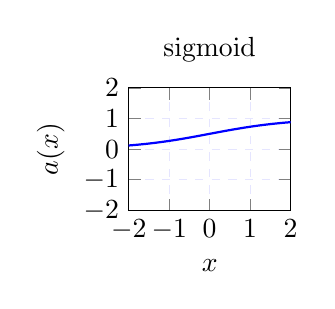
\begin{tikzpicture}
        \begin{axis}[
            title=sigmoid,
            width=0.3\linewidth, 
            grid=major,
            grid style={dashed, line width=.3pt, draw=presentblue!10},
            major grid style={line width=.3pt, draw=presentblue!10},
            xlabel={$x$},
            ylabel={$a(x)$},
            xmin=-2,
            xmax=2,
            ymin=-2,
            ymax=2
        ]
        \addplot [presentblue, thick, mark=none, smooth, samples=50] {1/(1+e^(-x))};
        \end{axis} 
    \end{tikzpicture}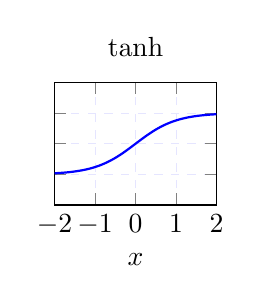
\begin{tikzpicture}
        \begin{axis}[
            title=tanh,
            width=0.3\linewidth, 
            grid=major,
            grid style={dashed, line width=.3pt, draw=presentblue!10},
            major grid style={line width=.3pt, draw=presentblue!10},
            yticklabels={,,},
            xlabel={$x$},
            xmin=-2,
            xmax=2,
            ymin=-2,
            ymax=2
        ]
    \addplot [presentblue, thick, mark=none, smooth, samples=50] {tanh(x)};
    \end{axis}
    \end{tikzpicture}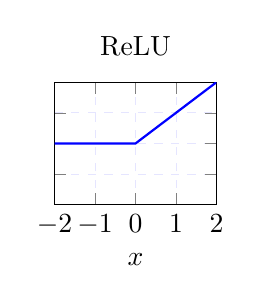
\begin{tikzpicture}
        \begin{axis}[
            title=ReLU,
            width=0.3\linewidth, 
            grid=major,
            grid style={dashed, line width=.3pt, draw=presentblue!10},
            major grid style={line width=.3pt, draw=presentblue!10},
            yticklabels={,,},
            xlabel={$x$},
            xmin=-2,
            xmax=2,
            ymin=-2,
            ymax=2
        ]
        \addplot [presentblue, thick, mark=none, domain=-3:3] {max(0, x)};
        \end{axis}
    \end{tikzpicture}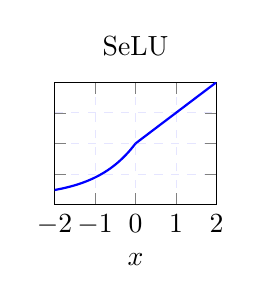
\begin{tikzpicture}
        \begin{axis}[
            title=SeLU,
            width=0.3\linewidth, 
            grid=major,
            grid style={dashed, line width=.3pt, draw=presentblue!10},
            major grid style={line width=.3pt, draw=presentblue!10},
            yticklabels={,,},
            xlabel={$x$},
            xmin=-2,
            xmax=2,
            ymin=-2,
            ymax=2
        ]
        \addplot [presentblue, thick, mark=none, smooth, samples=50, domain=-3:0]{1.0507 * 1.6732 * (e^x - 1)};
        \addplot [presentblue, thick, mark=none, smooth, samples=50, domain=0:3]{x};
        \end{axis}
    \end{tikzpicture}
    \end{figure}
\end{frame}

\begin{frame}
\frametitle{Universal Approximation Theorem}

\uncover<1->{
A feed-forward neural network with a linear output and at least one hidden layer can approximate any reasonable function to arbitrary precision with a finite number of nodes.
}
\vspace{0.5cm}
\begin{itemize}
    \item<2-> \textbf{Good News}
    \begin{itemize}
        \item Networks can perform highly complex tasks
        \item All necessary ingredients available
    \end{itemize}
    \item<3-> \textbf{Bad News}
    \begin{itemize}
        \item Does not specify number of necessary nodes
        \item No remarks on neuron connectivity
    \end{itemize}
\end{itemize}
\end{frame}

\begin{frame}
\frametitle{Deep Learning}

\begin{itemize}
    \item In practice: \textbf{stacking layers} works better
    \item \textbf{Deep learning:} more than one stage of non-linearities, e.g. layers
    \medskip
    \begin{figure}
        \centering
        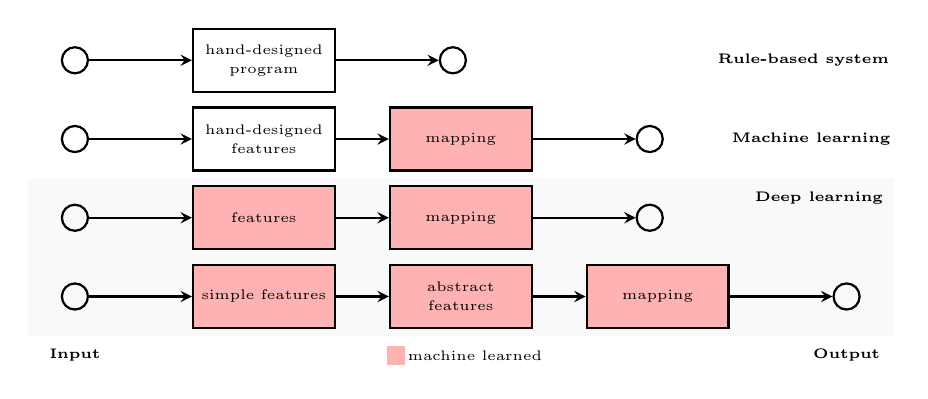
\begin{tikzpicture}
            \node[rectangle, fill=lightgray!10, minimum width=11cm, minimum height=2.0cm] at (4.0, 0.5) {};
        
            \node[draw, thick, circle, black] (input4) at (-0.9, 3) {};
            \node[draw, thick, circle, black] (input3) at (-0.9, 2) {};
            \node[draw, thick, circle, black] (input2) at (-0.9, 1) {};
            \node[draw, thick, circle, black] (input1) at (-0.9, 0) {};
            
            \node[draw, thick, rectangle, align=center, text width=1.6cm, minimum width=1.8cm, minimum height=0.8cm, inner sep=0cm] (node14) at (1.5, 3) {\tiny hand-designed\\[-5pt] program};
            \node[draw, thick, rectangle, align=center, minimum width=1.8cm, minimum height=0.8cm, inner sep=0cm] (node13) at (1.5, 2) {\tiny hand-designed\\[-5pt]\tiny features};
            \node[draw, thick, rectangle, align=center, minimum width=1.8cm, minimum height=0.8cm, inner sep=0cm, fill=presentred!30] (node12) at (1.5, 1) {\tiny features};
            \node[draw, thick, rectangle, align=center, minimum width=1.8cm, minimum height=0.8cm, inner sep=0cm, fill=presentred!30] (node11) at (1.5, 0) {\tiny simple features};
            
            \node[draw, thick, rectangle, align=center, minimum width=1.8cm, minimum height=0.8cm, inner sep=0cm, fill=presentred!30] (node23) at (4, 2) {\tiny mapping};
            \node[draw, thick, rectangle, align=center, minimum width=1.8cm, minimum height=0.8cm, inner sep=0cm, fill=presentred!30] (node22) at (4, 1) {\tiny mapping};
            \node[draw, thick, rectangle, align=center, minimum width=1.8cm, minimum height=0.8cm, inner sep=0cm, fill=presentred!30] (node21) at (4, 0) {\tiny abstract\\[-5pt]\tiny features};
            
            \node[draw, thick, rectangle, align=center, minimum width=1.8cm, minimum height=0.8cm, inner sep=0cm, fill=presentred!30] (node31) at (6.5, 0) {\tiny mapping};
            
            \node[draw, thick, circle, black] (output4) at (3.9, 3) {};
            \node[draw, thick, circle, black] (output3) at (6.4, 2) {};
            \node[draw, thick, circle, black] (output2) at (6.4, 1) {};
            \node[draw, thick, circle, black] (output1) at (8.9, 0) {};
            
            \draw[->, >=stealth, thick] (input4)--(node14);
            \draw[->, >=stealth, thick] (node14)--(output4);
            
            \draw[->, >=stealth, thick] (input3)--(node13);
            \draw[->, >=stealth, thick] (node13)--(node23);
            \draw[->, >=stealth, thick] (node23)--(output3);
            
            \draw[->, >=stealth, thick] (input2)--(node12);
            \draw[->, >=stealth, thick] (node12)--(node22);
            \draw[->, >=stealth, thick] (node22)--(output2);
            
            \draw[->, >=stealth, thick] (input1)--(node11);
            \draw[->, >=stealth, thick] (node11)--(node21);
            \draw[->, >=stealth, thick] (node21)--(node31);
            \draw[->, >=stealth, thick] (node31)--(output1);
            
            \node[] at (-0.9, -0.75) {\tiny\bfseries Input};
            \node[] at ( 8.9, -0.75) {\tiny\bfseries Output};
            \node[align=right] at (8.35, 3) {\tiny\bfseries Rule-based system};
            \node[align=right] at (8.45, 2) {\tiny\bfseries Machine learning};
            \node[align=right] at (8.55, 1.25) {\tiny\bfseries Deep learning};
            
            \node[fill=presentred!30] at (3.18, -0.75) {};
            \node[] at (4.18, -0.75) {\tiny machine learned};
        \end{tikzpicture}
    \end{figure}
\end{itemize}
\end{frame}

\subsection{Multi-class Classification}
\label{subsec:multi-class-classification}

\begin{frame}
\frametitle{Multi-class Classification}

\begin{columns}
    \begin{column}{0.48\textwidth}
        \begin{figure}
            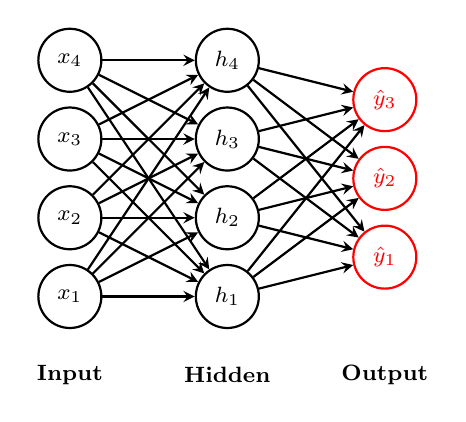
\begin{tikzpicture}
            \node[draw, circle, thick, minimum size=0.8cm] (input1) at (-2,-1.5) {\footnotesize$x_1$};
            \node[draw, circle, thick, minimum size=0.8cm] (input2) at (-2,-0.5) {\footnotesize$x_2$};
            \node[draw, circle, thick, minimum size=0.8cm] (input3) at (-2, 0.5) {\footnotesize$x_3$};
            \node[draw, circle, thick, minimum size=0.8cm] (input4) at (-2, 1.5) {\footnotesize$x_4$};
            
            \node[draw, circle, thick, minimum size=0.8cm] (hidden1) at (0,-1.5) {\footnotesize$h_1$};
            \node[draw, circle, thick, minimum size=0.8cm] (hidden2) at (0,-0.5) {\footnotesize$h_2$};
            \node[draw, circle, thick, minimum size=0.8cm] (hidden3) at (0, 0.5) {\footnotesize$h_3$};
            \node[draw, circle, thick, minimum size=0.8cm] (hidden4) at (0, 1.5) {\footnotesize$h_4$};
            
            \node[draw, presentred, circle, thick, minimum size=0.8cm] (output1) at (2, -1) {\footnotesize$\hat{y}_1$};
            \node[draw, presentred, circle, thick, minimum size=0.8cm] (output2) at (2, 0) {\footnotesize$\hat{y}_2$};
            \node[draw, presentred, circle, thick, minimum size=0.8cm] (output3) at (2, 1) {\footnotesize$\hat{y}_3$};
            
            \draw[->, >=stealth, thick] (input1)--(hidden1);
            \draw[->, >=stealth, thick] (input1)--(hidden2);
            \draw[->, >=stealth, thick] (input1)--(hidden3);
            \draw[->, >=stealth, thick] (input1)--(hidden4);
            
            \draw[->, >=stealth, thick] (input2)--(hidden1);
            \draw[->, >=stealth, thick] (input2)--(hidden2);
            \draw[->, >=stealth, thick] (input2)--(hidden3);
            \draw[->, >=stealth, thick] (input2)--(hidden4);
            
            \draw[->, >=stealth, thick] (input3)--(hidden1);
            \draw[->, >=stealth, thick] (input3)--(hidden2);
            \draw[->, >=stealth, thick] (input3)--(hidden3);
            \draw[->, >=stealth, thick] (input3)--(hidden4);
            
            \draw[->, >=stealth, thick] (input4)--(hidden1);
            \draw[->, >=stealth, thick] (input4)--(hidden2);
            \draw[->, >=stealth, thick] (input4)--(hidden3);
            \draw[->, >=stealth, thick] (input4)--(hidden4);
            
            \draw[->, >=stealth, thick] (hidden1)--(output1);
            \draw[->, >=stealth, thick] (hidden2)--(output1);
            \draw[->, >=stealth, thick] (hidden3)--(output1);
            \draw[->, >=stealth, thick] (hidden4)--(output1);
            
            \draw[->, >=stealth, thick] (hidden1)--(output2);
            \draw[->, >=stealth, thick] (hidden2)--(output2);
            \draw[->, >=stealth, thick] (hidden3)--(output2);
            \draw[->, >=stealth, thick] (hidden4)--(output2);
            
            \draw[->, >=stealth, thick] (hidden1)--(output3);
            \draw[->, >=stealth, thick] (hidden2)--(output3);
            \draw[->, >=stealth, thick] (hidden3)--(output3);
            \draw[->, >=stealth, thick] (hidden4)--(output3);
            
            \node at (-2, -2.5) {\footnotesize \textbf{Input}};
            \node at ( 0, -2.5) {\footnotesize \textbf{Hidden}};
            \node at ( 2, -2.5) {\footnotesize \textbf{Output}};
            \end{tikzpicture}
        \end{figure}
    \end{column}
    \begin{column}{0.48\textwidth}
        \begin{itemize}
            \item Extension of binary classification concept
            \item \textbf{One-versus-all classification}
            \begin{itemize}
                \item Build $c$ binary classifiers
                \item Pick class with highest confidence/probability
            \end{itemize}
            \item In neural networks
            \begin{itemize}
                \item Create multiple networks
                \item \textbf{Add output neurons}
            \end{itemize}
        \end{itemize}
    \end{column}
\end{columns}

\end{frame}

\begin{frame}
\frametitle{Multi-class Classification}

Multi-class classification recipe:
\medskip
\begin{itemize}
    \item \textbf{One-hot class encoding:} encode classes as sparse vectors \\
    $y=(y_1, y_2, ..., y_c)$, only one is active, e.g. class $2\rightarrow (0, 1, ..., 0)$
    \item \textbf{Softmax output activation:} $\hat{y}=softmax(z)=\frac{e^{z_{j}}}{\sum_{j}e^{z_{j}}}$ for $j=1...c$\\
    achieve joint-probability of $1$, normalize across model outputs $z$
    \item \textbf{Cross-entropy loss:} convex-function $J(w)=\frac{1}{n}\sum_{i=1}^{n}\sum_{j}^{c}y_{i,j}\log\hat{y}_{i,j}$\\
    maximum likelihood principle
\end{itemize}
\end{frame}

\subsection{Generalization}
\label{subsec:generalization}

\begin{frame}
\frametitle{Over- and Underfitting}

\begin{columns}
    \begin{column}{0.48\textwidth}
        \begin{figure}
            
\begin{tikzpicture}
            \begin{axis}[
                width=0.9\linewidth, 
                height=0.48\textheight,
                grid=both,
                grid style={line width=.3pt, draw=presentblue!10},
                major grid style={line width=.3pt, draw=presentblue!10},
                minor tick num=2,
                ticks=none,
                xticklabels={,,},
                ylabel={$y$},
                xmin=-0.1,
                xmax=1.0,
                ymin=-1.1,
                ymax=1.1
            ]
            \addplot [presentblue, thick, mark=none, smooth, samples=200] {sin(deg(2*pi*x))};
            \addplot [presentred, thick, mark=none] {0.036};
            \addplot [black, only marks, mark size=1pt, mark=*] coordinates {
                (0.0, 0.5)
                (0.1111111111111111, 0.6527876096865393)
                (0.2222222222222222, 0.984807753012208)
                (0.3333333333333333, 0.8960254037844387)
                (0.4444444444444444, 0.0)
                (0.5555555555555556, 0.07)
                (0.6666666666666666, -0.8660254037844384)
                (0.7777777777777777, -0.7848077530122082)
                (0.8888888888888888, -0.6427876096865396)
                (1.0, 0.0)
            };
            \node [] at (axis cs:0.85, 0.9) {\tiny degree=0};
            \end{axis} 
            \end{tikzpicture}
        \end{figure}\begin{figure}
            \begin{tikzpicture}
            \begin{axis}[
                width=0.9\linewidth, 
                height=0.48\textheight,
                grid=both,
                grid style={line width=.3pt, draw=presentblue!10},
                major grid style={line width=.3pt, draw=presentblue!10},
                minor tick num=2,
                ticks=none,
                xticklabels={,,},
                xlabel={$x$},
                ylabel={$y$},
                xmin=-0.1,
                xmax=1.0,
                ymin=-1.1,
                ymax=1.1
            ]
            \addplot [presentblue, thick, mark=none, smooth, samples=200] {sin(deg(2*pi*x))};
            \addplot [presentred, thick, mark=none, smooth, samples=200, domain=0:1] {18.6580627*x^3-28.0637985*x^2+9.40931656*x+0.0228460191};
            \addplot [black, only marks, mark size=1pt, mark=*] coordinates {
                (0.0, 0.5)
                (0.1111111111111111, 0.6527876096865393)
                (0.2222222222222222, 0.984807753012208)
                (0.3333333333333333, 0.8960254037844387)
                (0.4444444444444444, 0.0)
                (0.5555555555555556, 0.07)
                (0.6666666666666666, -0.8660254037844384)
                (0.7777777777777777, -0.7848077530122082)
                (0.8888888888888888, -0.6427876096865396)
                (1.0, 0.0)
            };
            \node [] at (axis cs:0.85, 0.9) {\tiny degree=3};
            \end{axis} 
            \end{tikzpicture}
        \end{figure}
    \end{column}
    \begin{column}{0.48\textwidth}
        \begin{figure}
            \begin{tikzpicture}
            \begin{axis}[
                width=0.9\linewidth, 
                height=0.48\textheight,
                grid=both,
                grid style={line width=.3pt, draw=presentblue!10},
                major grid style={line width=.3pt, draw=presentblue!10},
                minor tick num=2,
                ticks=none,
                xticklabels={,,},
                xmin=-0.1,
                xmax=1.0,
                ymin=-1.1,
                ymax=1.1
            ]
            \addplot [presentblue, thick, mark=none, smooth, samples=200] {sin(deg(2*pi*x))};
            \addplot [presentred, thick, mark=none, smooth, samples=10] {-1.28635944*x+0.67917972};
            \addplot [black, only marks, mark size=1pt, mark=*] coordinates {
                (0.0, 0.5)
                (0.1111111111111111, 0.6527876096865393)
                (0.2222222222222222, 0.984807753012208)
                (0.3333333333333333, 0.8960254037844387)
                (0.4444444444444444, 0.0)
                (0.5555555555555556, 0.07)
                (0.6666666666666666, -0.8660254037844384)
                (0.7777777777777777, -0.7848077530122082)
                (0.8888888888888888, -0.6427876096865396)
                (1.0, 0.0)
            };
            \node [] at (axis cs:0.85, 0.9) {\tiny degree=1};
            \end{axis} 
            \end{tikzpicture}
        \end{figure}\begin{figure}
            \begin{tikzpicture}
            \begin{axis}[
                width=0.9\linewidth, 
                height=0.48\textheight,
                grid=both,
                grid style={line width=.3pt, draw=presentblue!10},
                major grid style={line width=.3pt, draw=presentblue!10},
                minor tick num=2,
                ticks=none,
                xticklabels={,,},
                xlabel={$x$},
                xmin=-0.1,
                xmax=1.0,
                ymin=-1.1,
                ymax=1.1
            ]
            \addplot [presentblue, thick, mark=none, smooth, samples=200] {sin(deg(2*pi*x))};
            \addplot [presentred, thick, mark=none, smooth, samples=400, domain=0:1] {111819.288*x^9-500987.486*x^8+941671.207*x^7-964004.431*x^6+583394.102*x^5-211630.179*x^4+44379.6659*x^3-4855.25776*x^2+213.040344*x+0.0500000001};
            \addplot [black, only marks, mark size=1pt, mark=*] coordinates {
                (0.0, 0.5)
                (0.1111111111111111, 0.6527876096865393)
                (0.2222222222222222, 0.984807753012208)
                (0.3333333333333333, 0.8960254037844387)
                (0.4444444444444444, 0.0)
                (0.5555555555555556, 0.07)
                (0.6666666666666666, -0.8660254037844384)
                (0.7777777777777777, -0.7848077530122082)
                (0.8888888888888888, -0.6427876096865396)
                (1.0, 0.0)
            };
            \node [] at (axis cs:0.85, 0.9) {\tiny degree=9};
            \end{axis} 
            \end{tikzpicture}
        \end{figure}
    \end{column}
\end{columns}
\end{frame}

\begin{frame}
\frametitle{Over- and Underfitting}

\begin{itemize}
    \item How do we know a network is not over- or underfitting?
    \item \textbf{Idea:} simulate ``unseen'' data
    \item Split data artificially into disjoint subsets
    \begin{itemize}
        \item \textbf{Training set} for training the model (usually $60\%-80\%$)
        \item \textbf{Validation set} for fine tunine the model (usually $20\%$)
        \item \textbf{Test set} to test validation (usually $20\%-40\%$)
    \end{itemize}
\end{itemize}
\end{frame}

\begin{frame}
\frametitle{Over- and Underfitting}

\begin{columns}
    \begin{column}{0.48\textwidth}
        \begin{figure}
            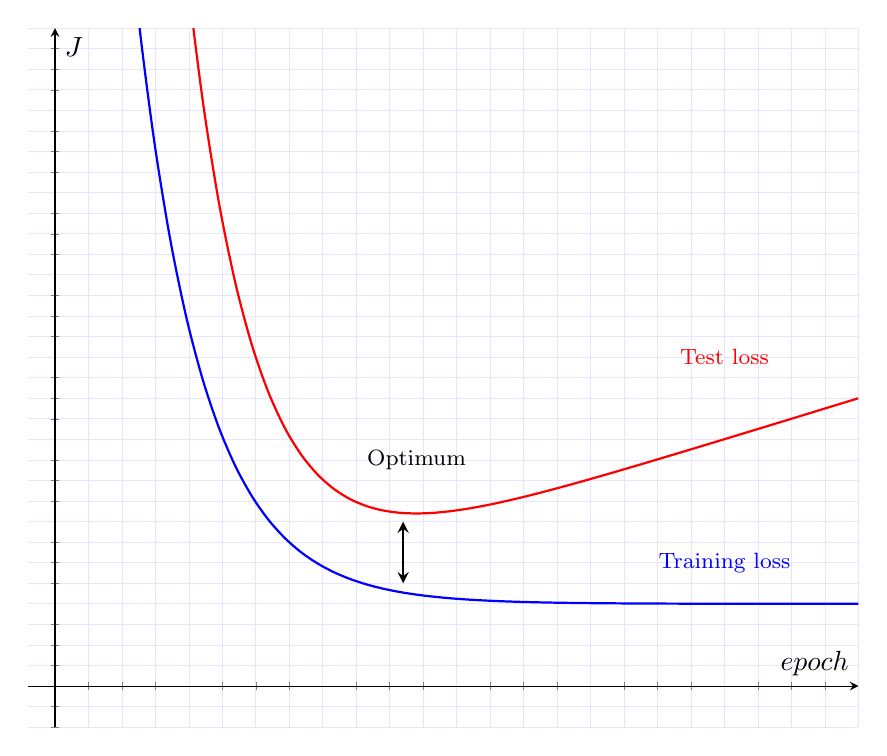
\begin{tikzpicture}
            \begin{axis}[
                width=\linewidth, 
                grid=both,
                grid style={line width=.3pt, draw=presentblue!10},
                major grid style={line width=.3pt, draw=presentblue!10},
                minor tick num=3,
                xlabel={$epoch$},
                ylabel={$J$}, 
                ticks=none,
                axis x line=center,
                axis y line=center,
                xmin=-0.1,
                xmax=3.0,
                ymin=-0.1,
                ymax=1.6
            ]
            % domain=0.25:2.75
            \addplot [presentred, thick, mark=none, smooth, samples=50, domain=0:3] {e^(-4*(x-0.6)) + 0.1 + 0.2*x};
            \addplot [presentblue, thick, mark=none, smooth, samples=50, domain=0:3] {e^(-4*(x-0.4)) + 0.2};
            \draw[<->, black, >=stealth, thick] (axis cs:1.3,0.25)--(axis cs:1.3,0.4);
            \node at (axis cs:2.5,0.8) [presentred]  {\footnotesize Test loss};
            \node at (axis cs:2.5,0.3) [presentblue] {\footnotesize Training loss};
            \node at (axis cs:1.35,0.55) [black] {\footnotesize Optimum};
            \end{axis} 
            \end{tikzpicture}
        \end{figure}
    \end{column}
    \begin{column}{0.48\textwidth}
        \begin{itemize}
            \item Separate monitoring of training and test loss during training
            \item Training loss will decrease indefinitely\\ $J\rightarrow 0$, \textbf{memorization effect}
            \item \textbf{Test loss minimum} is optimal
        \end{itemize}
    \end{column}
\end{columns}
\end{frame}

\begin{frame}
\frametitle{Regularization}

Methods to avoid overfitting, reduced validation error, might increase train error
\medskip
\begin{itemize}
    \item More data
    \item Augment: generate artificially new samples (add noise, translate, ...)
    \item Early stopping: monitoring of train and test loss, stop at optimum
    \item Penalize large weights: add a penalty term
    \item Dropout neurons
    \item Batch Normalization neurons
\end{itemize}
\end{frame}

\begin{frame}
    \frametitle{Penalty Terms}
    
    \begin{itemize}
        \item Weights can become increasingly large, allowing overfitting
        \item \textbf{Idea:} penalize large weights
        \item Minimize function $J^{*}(w)=J(w)+\lambda\Omega (w)$
        \item $\Omega (w)$ is measure of weight magnitude
        \item $\lambda$ is scale for $\Omega (w)$
        \begin{itemize}
            \item $J(w)\gg\lambda\Omega (w)$---no regularization
            \item $J(w)\ll\lambda\Omega (w)$---no training
        \end{itemize}
    \end{itemize}
\end{frame}

\begin{frame}
\frametitle{L1- and L2-Norm}

\begin{columns}
    \begin{column}{0.48\textwidth}
        \begin{itemize}
            \item \textbf{L1-Norm}, also \textbf{LASSO}
            \begin{itemize}
                \item $\lVert w\rVert_1=(w_1+w_2+\dots +w_f)$
                \item All weights contribute to loss
                \item Encourages sparsity
            \end{itemize}
            \item \textbf{L2-Norm}, also \textbf{weight decay}
            \begin{itemize}
                \item $\lVert w\rVert^2_2=(w_1^2+w_2^2+\dots +w_f^2)$
                \item Penalizes large weights
                \item Discourages sparsity
            \end{itemize}
        \end{itemize}
    \end{column}
    \begin{column}{0.48\textwidth}
        \begin{figure}
            \centering
            \begin{tikzpicture}
            \begin{axis}[
                width=0.7\textwidth, 
                height=0.55\textheight, 
                grid=both,
                grid style={line width=.3pt, draw=presentblue!10},
                major grid style={line width=.3pt, draw=presentblue!10},
                minor tick num=3,
                xlabel={$w_1$},
                ylabel={$w_2$}, 
                ticks=none,
                axis x line=center,
                axis y line=center,
                xmin=-2,
                xmax=2,
                ymin=-2,
                ymax=2
            ]
            \node[draw, thick, presentblue, minimum height=0.6cm, minimum width=0.6cm, rotate=45] at (axis cs: 0,0) {};
            \node[draw, thick, presentblue, minimum height=1.2cm, minimum width=1.2cm, rotate=45] at (axis cs: 0,0) {};
            \node[draw, thick, presentblue, minimum height=1.8cm, minimum width=1.8cm, rotate=45] at (axis cs: 0,0) {};
            \end{axis}
            \end{tikzpicture}\\\medskip
            \begin{tikzpicture}
            \begin{axis}[
                width=0.7\textwidth, 
                height=0.55\textheight, 
                grid=both,
                grid style={line width=.3pt, draw=presentblue!10},
                major grid style={line width=.3pt, draw=presentblue!10},
                minor tick num=3,
                xlabel={$w_1$},
                ylabel={$w_2$}, 
                ticks=none,
                axis x line=center,
                axis y line=center,
                xmin=-2,
                xmax=2,
                ymin=-2,
                ymax=2
            ]
            \draw[thick, presentblue] (axis cs: 0, 0) circle[radius=0.5];
            \draw[thick, presentblue] (axis cs: 0, 0) circle[radius=1.0];
            \draw[thick, presentblue] (axis cs: 0, 0) circle[radius=1.5];
            \end{axis}
            \end{tikzpicture}
        \end{figure}
    \end{column}
\end{columns}
\end{frame}

\begin{frame}
\frametitle{Dropout}

\begin{itemize}
    \item Randomly turn of neurons and connection, e.g. $p(drop)=0.5$
    \item Equivalent to network regularization (proof omitted)
\end{itemize}

\begin{columns}
    \begin{column}{0.48\textwidth}
        \begin{figure}
            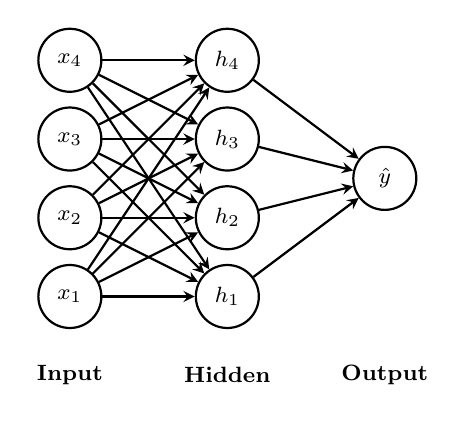
\begin{tikzpicture}
            \node[draw, circle, thick, minimum size=0.8cm] (input1) at (-2,-1.5) {\footnotesize$x_1$};
            \node[draw, circle, thick, minimum size=0.8cm] (input2) at (-2,-0.5) {\footnotesize$x_2$};
            \node[draw, circle, thick, minimum size=0.8cm] (input3) at (-2, 0.5) {\footnotesize$x_3$};
            \node[draw, circle, thick, minimum size=0.8cm] (input4) at (-2, 1.5) {\footnotesize$x_4$};
            
            \node[draw, circle, thick, minimum size=0.8cm] (hidden1) at (0,-1.5) {\footnotesize$h_1$};
            \node[draw, circle, thick, minimum size=0.8cm] (hidden2) at (0,-0.5) {\footnotesize$h_2$};
            \node[draw, circle, thick, minimum size=0.8cm] (hidden3) at (0, 0.5) {\footnotesize$h_3$};
            \node[draw, circle, thick, minimum size=0.8cm] (hidden4) at (0, 1.5) {\footnotesize$h_4$};
            
            \node[draw, circle, thick, minimum size=0.8cm] (output) at (2, 0) {\footnotesize$\hat{y}$};
            
            \draw[->, >=stealth, thick] (input1)--(hidden1);
            \draw[->, >=stealth, thick] (input1)--(hidden2);
            \draw[->, >=stealth, thick] (input1)--(hidden3);
            \draw[->, >=stealth, thick] (input1)--(hidden4);
            
            \draw[->, >=stealth, thick] (input2)--(hidden1);
            \draw[->, >=stealth, thick] (input2)--(hidden2);
            \draw[->, >=stealth, thick] (input2)--(hidden3);
            \draw[->, >=stealth, thick] (input2)--(hidden4);
            
            \draw[->, >=stealth, thick] (input3)--(hidden1);
            \draw[->, >=stealth, thick] (input3)--(hidden2);
            \draw[->, >=stealth, thick] (input3)--(hidden3);
            \draw[->, >=stealth, thick] (input3)--(hidden4);
            
            \draw[->, >=stealth, thick] (input4)--(hidden1);
            \draw[->, >=stealth, thick] (input4)--(hidden2);
            \draw[->, >=stealth, thick] (input4)--(hidden3);
            \draw[->, >=stealth, thick] (input4)--(hidden4);
            
            \draw[->, >=stealth, thick] (hidden1)--(output);
            \draw[->, >=stealth, thick] (hidden2)--(output);
            \draw[->, >=stealth, thick] (hidden3)--(output);
            \draw[->, >=stealth, thick] (hidden4)--(output);
            
            \node at (-2, -2.5) {\footnotesize \textbf{Input}};
            \node at ( 0, -2.5) {\footnotesize \textbf{Hidden}};
            \node at ( 2, -2.5) {\footnotesize \textbf{Output}};
            \end{tikzpicture}
        \end{figure}
    \end{column}
    \begin{column}{0.48\textwidth}
        \begin{figure}
            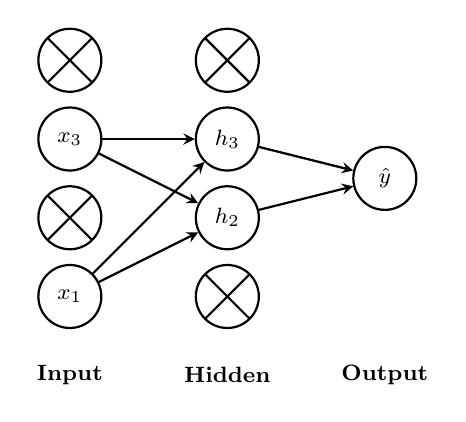
\begin{tikzpicture}
            \node[draw, circle, thick, minimum size=0.8cm] (input1) at (-2,-1.5) {\footnotesize$x_1$};
            \node[draw, cross, circle, thick, minimum size=0.8cm] (input2) at (-2,-0.5) {};
            \node[draw, circle, thick, minimum size=0.8cm] (input3) at (-2, 0.5) {\footnotesize$x_3$};
            \node[draw, cross, circle, thick, minimum size=0.8cm] (input4) at (-2, 1.5) {};
            
            \node[draw, cross, circle, thick, minimum size=0.8cm] (hidden1) at (0,-1.5) {};
            \node[draw, circle, thick, minimum size=0.8cm] (hidden2) at (0,-0.5) {\footnotesize$h_2$};
            \node[draw, circle, thick, minimum size=0.8cm] (hidden3) at (0, 0.5) {\footnotesize$h_3$};
            \node[draw, cross, circle, thick, minimum size=0.8cm] (hidden4) at (0, 1.5) {};
            
            \node[draw, circle, thick, minimum size=0.8cm] (output) at (2, 0) {\footnotesize$\hat{y}$};
            
            \draw[->, >=stealth, thick] (input1)--(hidden2);
            \draw[->, >=stealth, thick] (input1)--(hidden3);
            
            \draw[->, >=stealth, thick] (input3)--(hidden2);
            \draw[->, >=stealth, thick] (input3)--(hidden3);
            
            \draw[->, >=stealth, thick] (hidden2)--(output);
            \draw[->, >=stealth, thick] (hidden3)--(output);
            
            \node at (-2, -2.5) {\footnotesize \textbf{Input}};
            \node at ( 0, -2.5) {\footnotesize \textbf{Hidden}};
            \node at ( 2, -2.5) {\footnotesize \textbf{Output}};
            \end{tikzpicture}
        \end{figure}
    \end{column}
\end{columns}
\end{frame}

\begin{frame}[fragile]
\frametitle{Neural Networks in Keras}

\begin{lstlisting}[language=Python]
from keras.models import Sequential
from keras.layers import Dense, Dropout
from keras.regularizers import l2

classes, features = 10, 200

# Fully-connected neural network
model = Sequential()
model.add(Dense(16, input_dim=features, activation="tanh"))
model.add(Dense(16, kernel_regularizer=l2(0.02))
model.add(Dropout(0.1))
model.add(Dense(classes, activation='softmax'))

# Model compilation
model.compile(loss="categorical_crossentropy", optimizer="sgd")
\end{lstlisting}

\end{frame}

\subsection{Exercise: MNIST FNN}
\label{subsec:exercise-fnn}

\begin{frame}
    \frametitle{Exercise: FNN MNIST Image Classification}
    
    \begin{figure}
        \centering
        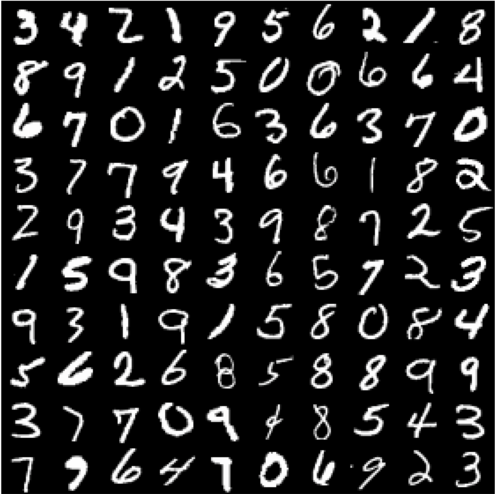
\includegraphics[width=0.4\linewidth]{mnist.png}
    \end{figure}
\end{frame}

\section{Convolutional Neural Networks}
\label{sec:convolutional-neural-networks}

\subsection{Deep Learning}
\label{subsec:deep-learning}

\subsection{Discrete Convolution}
\label{subsec:discrete-convolution}

\begin{frame}
\frametitle{Computer Vision}

\begin{columns}
    \begin{column}{0.48\textwidth}
        \begin{figure}
            \centering
            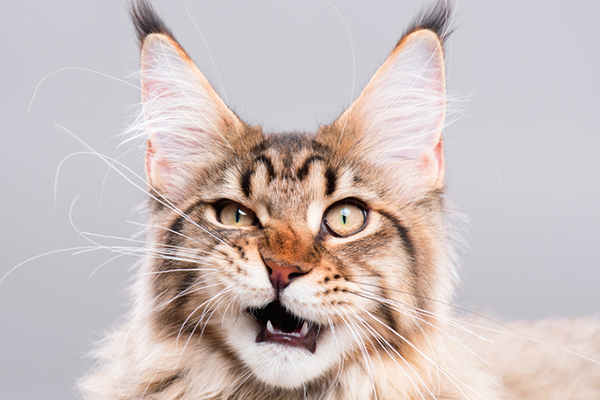
\includegraphics[width=\linewidth]{cat.jpg}
            \imageright{Catster}
        \end{figure}
    \end{column}
    \begin{column}{0.48\textwidth}
        \begin{itemize}
            \item Easy for humans, hard for machines
            \item High input dimensionality $\mathbb{R}/\mathbb{N}^{10^1-10^8}$
            \item Have to deal with POV-shifts, light variation, occlusion, shape variation
            \item Classical computer vision answer:
            \begin{itemize}
                \item Inclusion of context information
                \item Usage of image filters
            \end{itemize}
            \item \textbf{Idea:} combine with machine learning
        \end{itemize}
    \end{column}
\end{columns}
\end{frame}

\begin{frame}
\frametitle{Discrete Convolution}

\begin{columns}
    \begin{column}{0.58\textwidth}
        \begin{itemize}
            \item Element-wise weighted sum of input and filter
            \item $(f*g)[n]=\sum_{m=-\infty}^{\infty}f[m]g[n-m]$
            \item \textbf{Stride:} pixel distance for slide
            \item \textbf{Filter size:} window size of convolution kernel
            \item 2D input: volume of $width\times height(\times channels)$
            \item Models effects on images, e.g. edge detection
            \item In CNN: model ``eye'', sparse weight sharing
        \end{itemize}
    \end{column}
    \begin{column}{0.38\textwidth}
        \begin{figure}
            \centering
            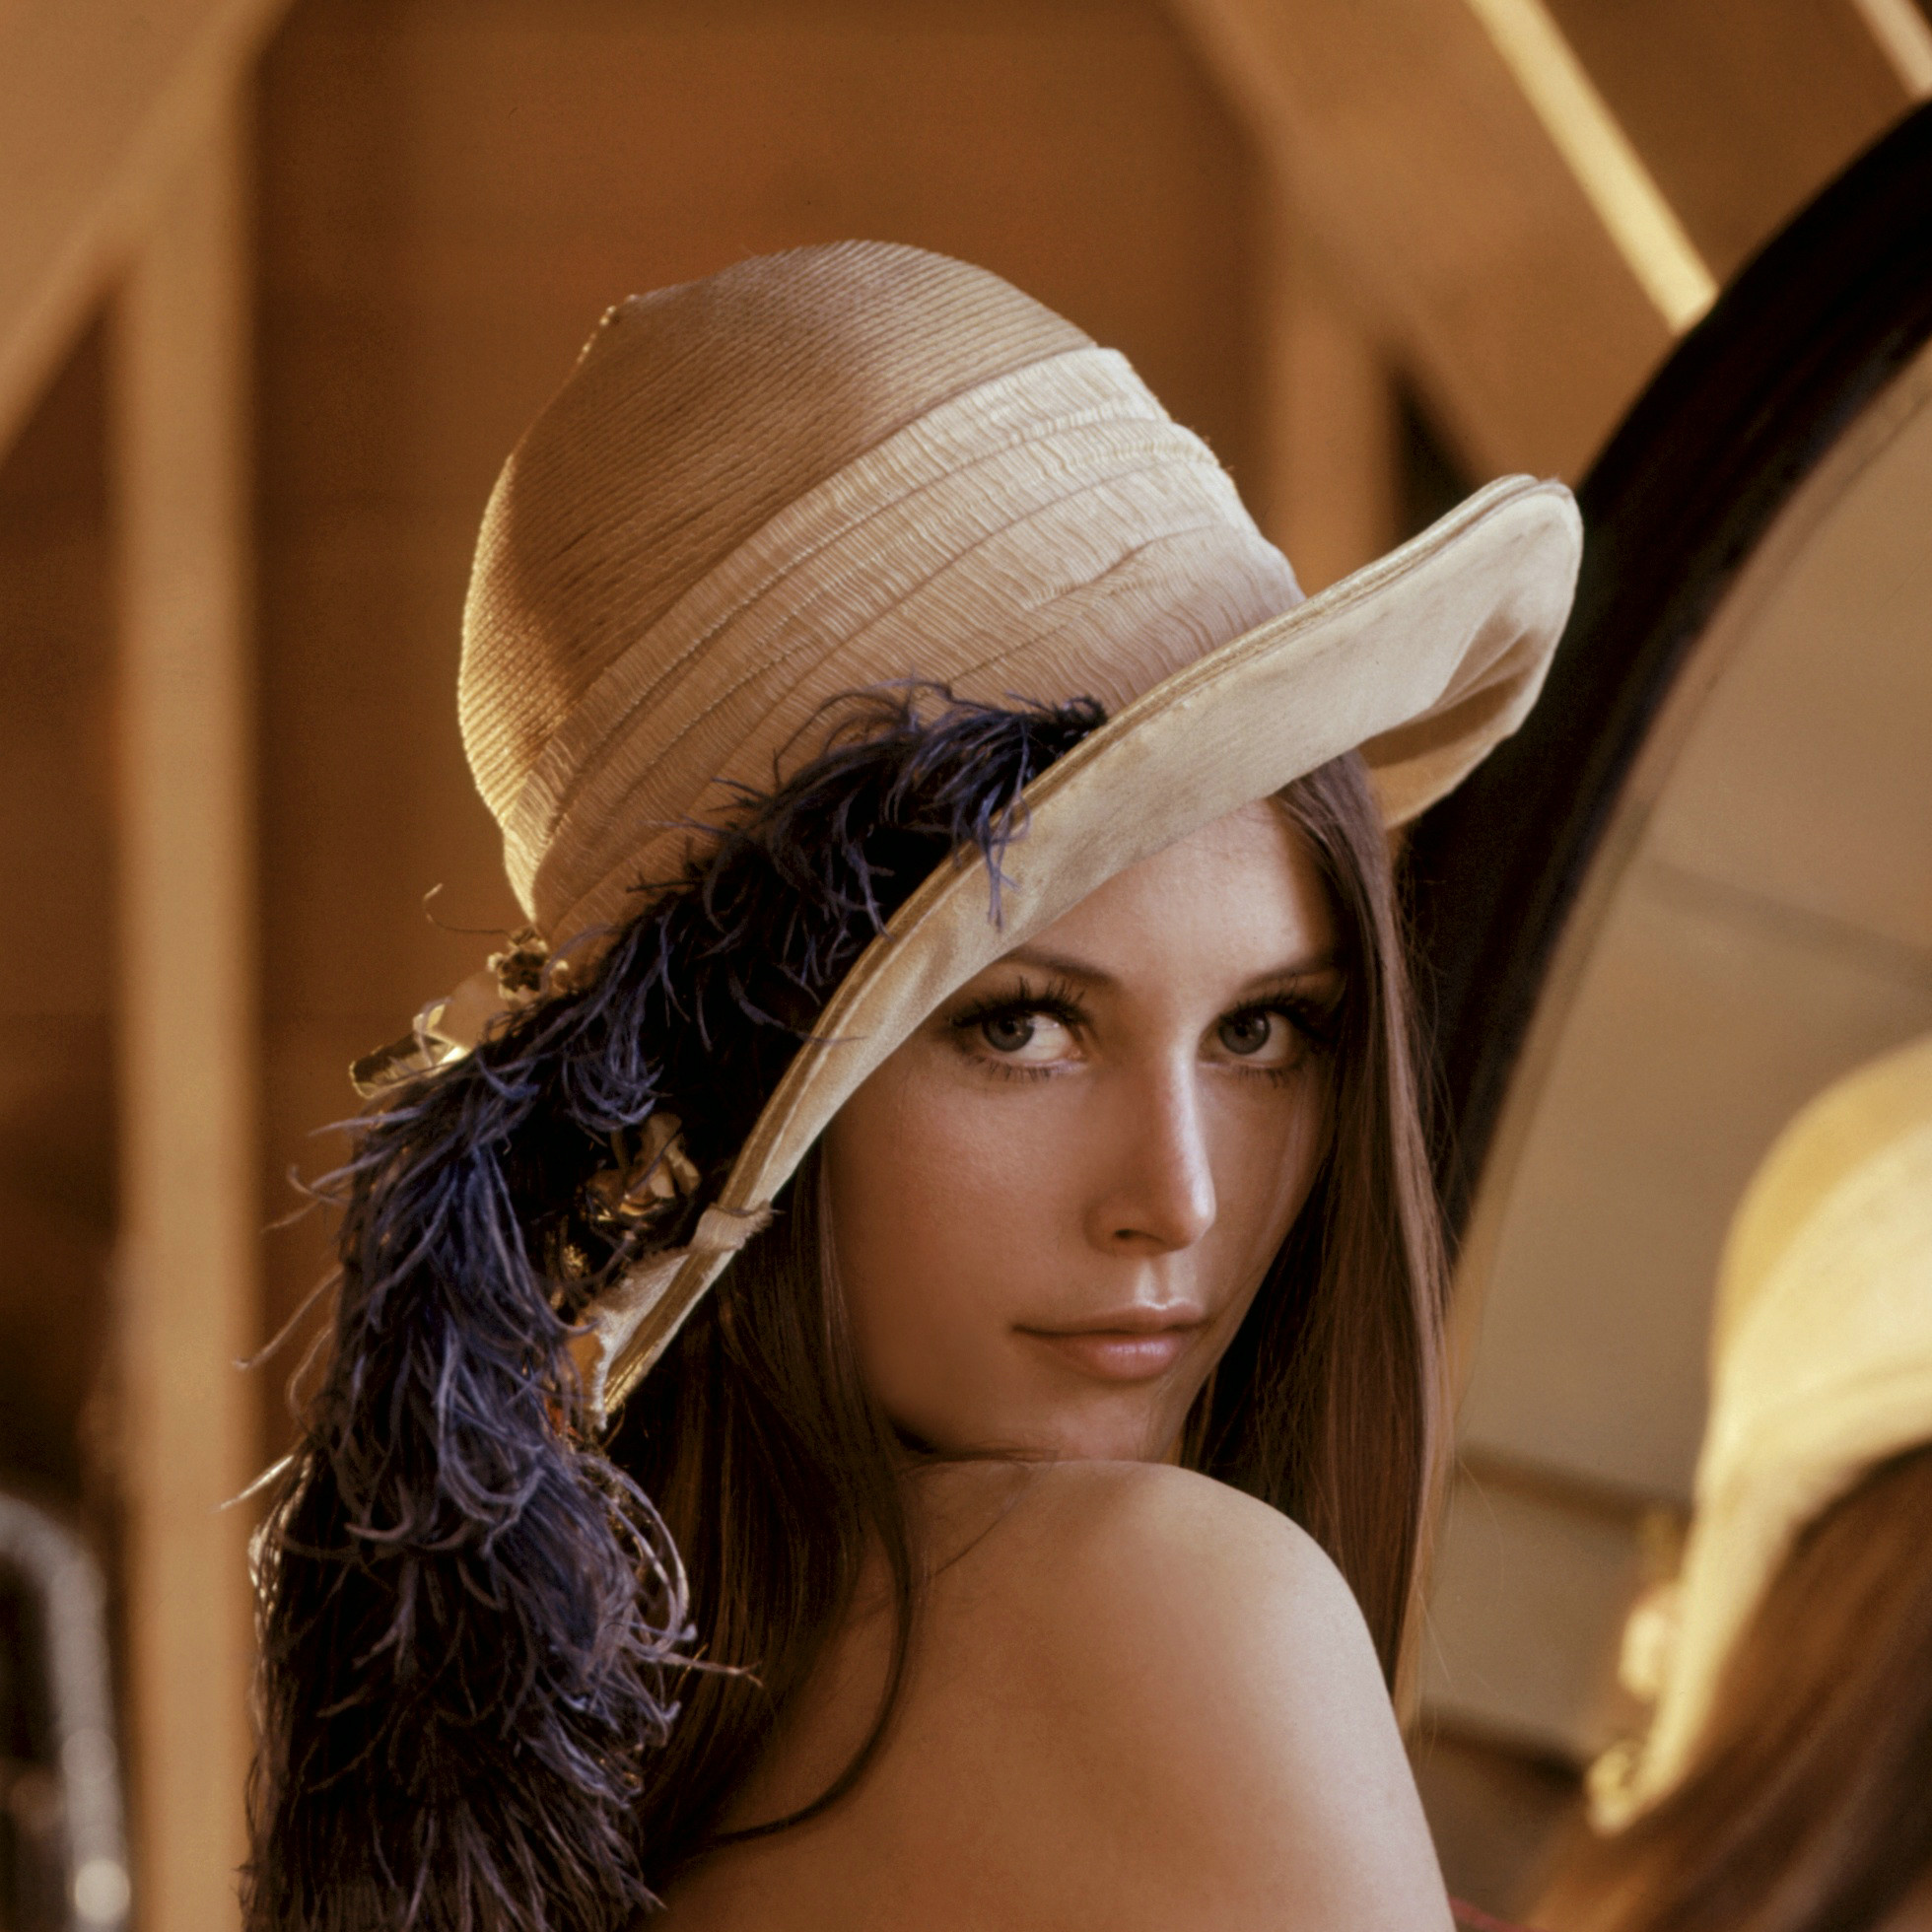
\includegraphics[height=0.38\textheight]{lena.jpg}\\
            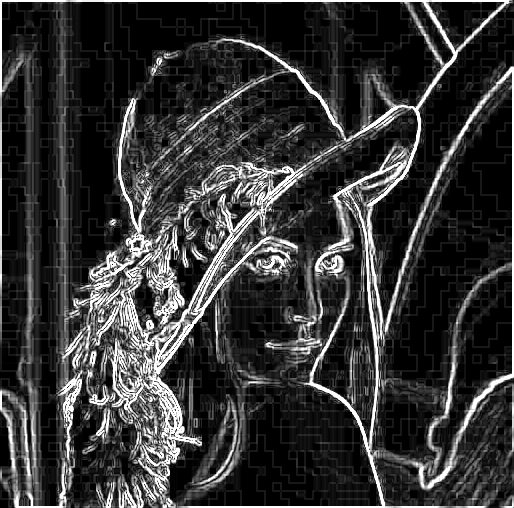
\includegraphics[height=0.38\textheight]{sobel.png}
        \end{figure}
    \end{column}
\end{columns}
\end{frame}

\begin{frame}
    \frametitle{Discrete Convolution}
    \begin{figure}
        \centering
        \multiinclude[<+->][format=png, graphics={width=0.8\linewidth}]{convolution}
        \imageright{Machine Learning Guru}
    \end{figure}
\end{frame}

\begin{frame}
\frametitle{Pooling}

\begin{columns}
    \begin{column}{0.48\textwidth}
        \begin{itemize}
            \item \textbf{Pooling} reduces input sizes, \\
            abstract downsampled copy
            \item \textbf{Pool size:} kernel height/width
            \item \textbf{Strides:} step width
            \item Typical pooling layers
            \begin{itemize}
                \item Max Pooling
                \item Average Pooling
            \end{itemize}
        \end{itemize}
    \end{column}
    \begin{column}{0.48\textwidth}
        \begin{figure}
            \centering
            \resizebox{!}{0.7\textheight}{
            \begin{tikzpicture}
                \node[draw, fill=presentblue!30, rectangle, minimum width=1cm, minimum height=1cm] (1) at (0,0) {1};
                \node[draw, fill=presentblue!30, rectangle, minimum width=1cm, minimum height=1cm] (2) at (1,0) {1};
                \node[draw, fill=presentblue!30, rectangle, minimum width=1cm, minimum height=1cm] (3) at (0,1) {4};
                \node[draw, fill=presentblue!30, rectangle, minimum width=1cm, minimum height=1cm] (4) at (1,1) {6};
                
                \node[draw, fill=hgfgreen!30, rectangle, minimum width=1cm, minimum height=1cm] (5) at (2,0) {2};
                \node[draw, fill=hgfgreen!30, rectangle, minimum width=1cm, minimum height=1cm] (6) at (3,0) {4};
                \node[draw, fill=hgfgreen!30, rectangle, minimum width=1cm, minimum height=1cm] (7) at (2,1) {7};
                \node[draw, fill=hgfgreen!30, rectangle, minimum width=1cm, minimum height=1cm] (8) at (3,1) {8};
                
                \node[draw, fill=presentred!30, rectangle, minimum width=1cm, minimum height=1cm] (9) at (0,2) {3};
                \node[draw, fill=presentred!30, rectangle, minimum width=1cm, minimum height=1cm] (10) at (1,2) {2};
                \node[draw, fill=presentred!30, rectangle, minimum width=1cm, minimum height=1cm] (11) at (0,3) {1};
                \node[draw, fill=presentred!30, rectangle, minimum width=1cm, minimum height=1cm] (12) at (1,3) {1};
                
                \node[draw, fill=hgfaero!30, rectangle, minimum width=1cm, minimum height=1cm] (13) at (2,2) {1};
                \node[draw, fill=hgfaero!30, rectangle, minimum width=1cm, minimum height=1cm] (14) at (3,2) {0};
                \node[draw, fill=hgfaero!30, rectangle, minimum width=1cm, minimum height=1cm] (15) at (2,3) {3};
                \node[draw, fill=hgfaero!30, rectangle, minimum width=1cm, minimum height=1cm] (16) at (3,3) {4};
                
                
                \node[draw, fill=presentblue!30, rectangle, minimum width=1cm, minimum height=1cm] (13) at (1,-3) {6};
                \node[draw, fill=hgfgreen!30, rectangle, minimum width=1cm, minimum height=1cm] (14) at (2,-3) {8};
                \node[draw, fill=presentred!30, rectangle, minimum width=1cm, minimum height=1cm] (15) at (1,-2) {3};
                \node[draw, fill=hgfaero!30, rectangle, minimum width=1cm, minimum height=1cm] (16) at (2,-2) {4};
                
                \draw[->, >=stealth, thick] (1.5,-0.6)--(1.5,-1.4);
                \node[] at (3.2, -1.0) {\tiny\textbf{$2\times 2$ Max Pooling, stride $2\times 2$}};
            \end{tikzpicture}}
        \end{figure}
    \end{column}
\end{columns}
\end{frame}

\begin{frame}
\frametitle{Convolutional Neural Network Pyramid}

\begin{figure}
    \centering
    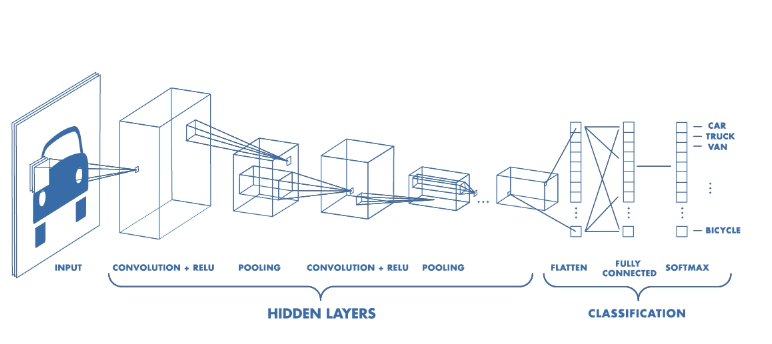
\includegraphics[width=\linewidth]{pyramid.png}
    \imageright{Medium}
\end{figure}
\end{frame}

\begin{frame}
\frametitle{Batch Normalization}

\begin{columns}
    \begin{column}{0.48\textwidth}
        \begin{itemize}
            \item \textbf{Idea:} standardize layer outputs
            \item Training time
            \begin{itemize}
                \item Calculate batch mean $\mu_B$ and standard deviation $\sigma_B$
                \item Track rolling values $\mu$ and $\sigma$
                \item Normalize by $\frac{x-\mu_B}{\sigma_B}$
            \end{itemize}
            \item Prediction time
            \begin{itemize}
                \item Track $\mu_B$ and $\sigma_B$ for covariate shift
                \item Add one degree of freedom
            \end{itemize}
            \item Regularizes network
        \end{itemize}
    \end{column}
    \begin{column}{0.48\textwidth}
        \begin{figure}
            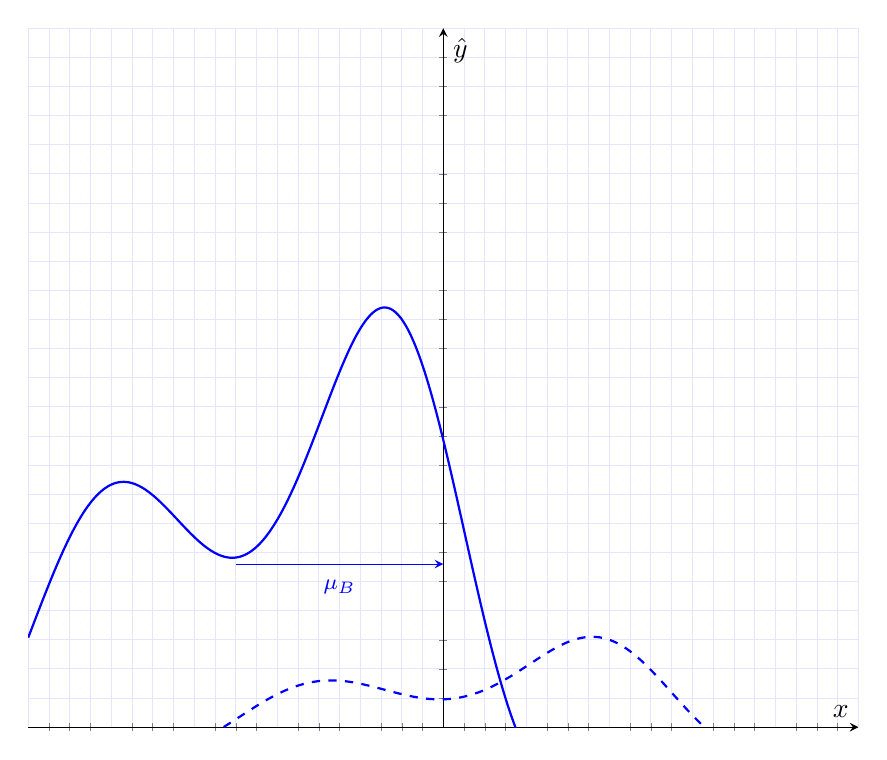
\begin{tikzpicture}
            \begin{axis}[
                width=\linewidth, 
                grid=both,
                grid style={line width=.3pt, draw=presentblue!10},
                major grid style={line width=.3pt, draw=presentblue!10},
                minor tick num=3,
                xlabel={$x$},
                ylabel={$\hat{y}$}, 
                axis x line=center,
                axis y line=center,
                ticks=none,
                xmin=-5,
                xmax=5,
                ymin=0.0,
                ymax=6.0,
            ]
            \addplot [presentblue, mark=none, thick, smooth, samples=100, domain=-5:1] {e^(-(x+0.5) ^2)-sin(deg(x+0.5)) + cos(1.69*deg(x+0.5)) + 1.5};
            \addplot [presentblue, dashed, mark=none, thick, smooth, samples=100,domain=-3:4] {(e^(-(x-2)^2)-sin(deg(x-2)) + cos(1.69*deg(x-2)) + 1)/4.0};
            \draw[presentblue, ->, >=stealth] (axis cs:-2.5,1.4)--(0,1.4);
            \node[presentblue] at (axis cs:-1.25,1.2) {\footnotesize$\mu_B$};
            \end{axis} 
            \end{tikzpicture}
        \end{figure}
    \end{column}
\end{columns}
\end{frame}

\begin{frame}
\frametitle{Optimizers}

\begin{columns}
    \begin{column}{0.48\textwidth}
        \begin{figure}
            \begin{tikzpicture}
            \begin{axis}[
                width=\linewidth, 
                grid=both,
                grid style={line width=.3pt, draw=presentblue!10},
                major grid style={line width=.3pt, draw=presentblue!10},
                minor tick num=3,
                xlabel={$epoch$},
                ylabel={$J$}, 
                axis x line=center,
                axis y line=center,
                ticks=none,
                xmin=0,
                xmax=5,
                ymin=0.0,
                ymax=1.5,
            ]
            \addplot [presentred, mark=none, thick, smooth,samples=100, domain=0:5] {(e^(-3*x)) + 0.2};
            \addplot [presentblue, mark=none, thick, smooth,samples=100, domain=0:5] {(e^(-x)) + 0.01};
            \addplot [hgfmatter, mark=none, thick, smooth,samples=100, domain=0:5] {(e^(-0.2*x)) + 0.01};
            \addplot [hgfee, mark=none, thick, smooth] {0.1*x+1.0};
            
            \node[presentred] at (axis cs:3.1,0.24) {\footnotesize high};
            \node[presentblue] at (axis cs:3.1,0.12) {\footnotesize optimal};
            \node[hgfmatter] at (axis cs:3.1,0.7) {\footnotesize too low};
            \node[hgfee] at (axis cs:3.1,1.1) {\footnotesize too high};
            \end{axis} 
            \end{tikzpicture}
        \end{figure}
    \end{column}
    \begin{column}{0.48\textwidth}
        \begin{itemize}
            \item Learning rate strongly impacts training
            \item Value for $lr$
            \begin{itemize}
                \item high: jumpy, no convergence
                \item low: slow training, local minima
            \end{itemize}
            \item Earlier approach 
            \begin{itemize}
                \item stop training every $e$ epochs
                \item lower $lr$
                \item continue training
            \end{itemize}
        \end{itemize}
    \end{column}
\end{columns}
\end{frame}

\begin{frame}
\frametitle{Optimizers}

\begin{columns}
\begin{column}{0.48\textwidth}
    \begin{itemize}
        \item Various flavors of SGD
        \item Include \textbf{gradient momentum}
        \begin{itemize}
            \item Accelerate previous gradient
            \item $J_{t+1}^{*}(w)=\alpha J_{t}^{*}(w) - lr\nabla J_t(w)$
        \end{itemize}
        \item \textbf{Adaptive learning rate}
        \begin{itemize}
            \item Implemented in \textbf{Adagrad}
            \item Learning rate $lr_i$ for each weight $w_i$
            \item $w_{i+1}=w_i \frac{lr_{t,i}}{\sqrt{\sum_{i=1}^{\infty} \nabla_{w_i}J_{t-i}(w_i)^2}}\nabla_{w_i} J_t(w_i)$
        \end{itemize}
    \end{itemize}
\end{column}
\begin{column}{0.48\textwidth}
    \begin{figure}
        \begin{tikzpicture}
        \begin{axis}[
            width=\linewidth, 
            height=0.48\textheight,
            grid=both,
            grid style={line width=.3pt, draw=presentblue!10},
            major grid style={line width=.3pt, draw=presentblue!10},
            minor tick num=2,
            xlabel={$w_1$},
            ylabel={$w_2$}, 
            axis x line=center,
            axis y line=center,
            ticks=none,
            xmin=-3,
            xmax=3,
            ymin=-2,
            ymax=2,
        ]
        \draw (0, 0) ellipse (2.2 and 1.5);
        \draw (0, 0) ellipse (1.7 and 1.0);
        \draw (0, 0) ellipse (1.2 and 0.5);
        \draw[->, >= stealth, presentblue] (axis cs:-2.1,0.8)--(axis cs:-1.9, -0.6) --(axis cs:-1.7, 0.5)--(axis cs:-1.5, -0.4)--(axis cs:-1.3, 0.3){};
        \end{axis} 
        \end{tikzpicture}\\
        \bigskip
        \begin{tikzpicture}
        \begin{axis}[
            width=\linewidth, 
            height=0.48\textheight,
            grid=both,
            grid style={line width=.3pt, draw=presentblue!10},
            major grid style={line width=.3pt, draw=presentblue!10},
            minor tick num=2,
            xlabel={$w_1$},
            ylabel={$w_2$}, 
            axis x line=center,
            axis y line=center,
            ticks=none,
            xmin=-3,
            xmax=3,
            ymin=-2,
            ymax=2,
        ]
        \draw (0, 0) ellipse (2.2 and 1.5);
        \draw (0, 0) ellipse (1.7 and 1.0);
        \draw (0, 0) ellipse (1.2 and 0.5);
        \draw[->, >= stealth, presentblue] (axis cs:-2.1,0.8)--(axis cs:-1.6, -0.5) --(axis cs:-1.1, 0.4)--(axis cs:-0.6, -0.3)--(axis cs:-0.1, 0.2){};
        \end{axis} 
        \end{tikzpicture}
    \end{figure}
\end{column}
\end{columns}
\end{frame}

\begin{frame}
\frametitle{Optimizers}

\begin{columns}
    \begin{column}{0.48\textwidth}
        \begin{figure}
            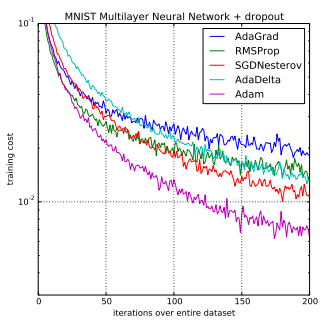
\includegraphics[width=\linewidth]{optimizers.png}
            \imageright{Machine Learning Mastery}
        \end{figure}
    \end{column}
    \begin{column}{0.48\textwidth}
        \begin{itemize}
            \item \textbf{RMSprop:} enhanced Adagrad
            \begin{itemize}
                \item Learning rate got infinitely small
                \item Forgetting factor $\beta$ for past gradients
            \end{itemize}
            \item More intricate variants: Nesterov momentum, Adadelta, Nadam, $\dots$
            \item Some \textbf{non-SGD} alternatives
            \begin{itemize}
                \item Particle-swarm optimization (PSO)
                \item BFGS
            \end{itemize}
        \end{itemize}
    \end{column}
\end{columns}
\end{frame}

\begin{frame}
\frametitle{Hyperparameter Optimization}

\begin{itemize}
    \item \textbf{Hyperparameters are all non-weight parameters}
    \begin{itemize}
        \item Optimization algorithm
        \item Learning rate
        \item Regularization
        \item Network layer count
        \item Network neurons
        \item $\dots$
    \end{itemize}
    \item Some can be inferred through thought
    \item \textbf{Rest: trial and error}
\end{itemize}
\end{frame}

\begin{frame}
\frametitle{Hyperparameter Optimization}

\begin{columns}
    \begin{column}{0.48\textwidth}
        \begin{itemize}
            \item Naïve approaches
            \begin{itemize}
                \item Grid search
                \item \textbf{Random search}
            \end{itemize}
            \item \textbf{Search} algorithms
            \begin{itemize}
                \item Kriging-based (hyperopt, Vizier)
                \item Particle-swarm optimization
                \item Genetic algorithms
            \end{itemize}
            \item \textbf{Meta-learning:} use NN to find NN
        \end{itemize}
    \end{column}
    \begin{column}{0.48\textwidth}
        \begin{figure}
            \centering
            \begin{tikzpicture}
            \begin{axis}[
                width=0.8\linewidth,
                height=0.4\textheight,
                grid=major,
                grid style={line width=.3pt, draw=presentblue!10},
                major grid style={line width=.3pt, draw=presentblue!10},
                yticklabels={,,},
                xticklabels={,,},
                ylabel={$x_2$},
                xmin=-1.9,
                xmax=1.9,
                ymin=-1.9,
                ymax=1.9,
                title={\footnotesize\textbf{grid search}}
            ]
            \node[draw, circle, fill=presentblue, minimum size=0.2cm, inner sep=0pt] at (-1, -1) {};
            \node[draw, circle, fill=presentblue, minimum size=0.2cm, inner sep=0pt] at ( 0, -1) {};
            \node[draw, circle, fill=presentblue, minimum size=0.2cm, inner sep=0pt] at ( 1, -1) {};
            \node[draw, circle, fill=presentblue, minimum size=0.2cm, inner sep=0pt] at (-1,  0) {};
            \node[draw, circle, fill=presentblue, minimum size=0.2cm, inner sep=0pt] at ( 0,  0) {};
            \node[draw, circle, fill=presentblue, minimum size=0.2cm, inner sep=0pt] at ( 1,  0) {};
            \node[draw, circle, fill=presentblue, minimum size=0.2cm, inner sep=0pt] at (-1,  1) {};
            \node[draw, circle, fill=presentblue, minimum size=0.2cm, inner sep=0pt] at ( 0,  1) {};
            \node[draw, circle, fill=presentblue, minimum size=0.2cm, inner sep=0pt] at ( 1,  1) {};
            \end{axis}
            \end{tikzpicture}\\\medskip
            \begin{tikzpicture}
            \begin{axis}[
                width=0.8\linewidth,
                height=0.43\textheight,
                grid=major,
                grid style={line width=.3pt, draw=presentblue!10},
                major grid style={line width=.3pt, draw=presentblue!10},
                yticklabels={,,},
                xticklabels={,,},
                ylabel={$x_2$},
                xlabel={$x_1$},
                xmin=-1.9,
                xmax=1.9,
                ymin=-1.9,
                ymax=1.9,
                title={\footnotesize\textbf{random search}}
            ]
            \node[draw, circle, fill=presentblue, minimum size=0.2cm, inner sep=0pt] at (-1,     0) {};
            \node[draw, circle, fill=presentblue, minimum size=0.2cm, inner sep=0pt] at (-0.75, -1) {};
            \node[draw, circle, fill=presentblue, minimum size=0.2cm, inner sep=0pt] at (-0.5,   1) {};
            \node[draw, circle, fill=presentblue, minimum size=0.2cm, inner sep=0pt] at (-0.25, -0.5) {};
            \node[draw, circle, fill=presentblue, minimum size=0.2cm, inner sep=0pt] at ( 0,    0.75) {};
            \node[draw, circle, fill=presentblue, minimum size=0.2cm, inner sep=0pt] at ( 0.25, 0.66) {};
            \node[draw, circle, fill=presentblue, minimum size=0.2cm, inner sep=0pt] at ( 0.5,  -0.3) {};
            \node[draw, circle, fill=presentblue, minimum size=0.2cm, inner sep=0pt] at ( 0.75,  0.2) {};
            \node[draw, circle, fill=presentblue, minimum size=0.2cm, inner sep=0pt] at ( 1,     0.8) {};
            \end{axis}
            \end{tikzpicture}
        \end{figure}
    \end{column}
\end{columns}
\end{frame}

\subsection{Network Architectures}
\label{subsec:network-architectures}

\begin{frame}
\frametitle{ImageNet Large Scale Visual Recognition Challenge (ILSVRC)}

\begin{columns}
    \begin{column}{0.48\textwidth}
        \begin{figure}
            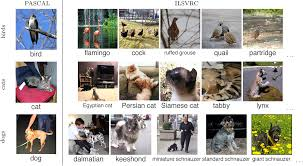
\includegraphics[width=\linewidth]{ilsvrc.jpg}
            \imageright{Oren Kraus}
        \end{figure}
    \end{column}
    \begin{column}{0.48\textwidth}
        \begin{itemize}
            \item \textbf{Main image recognition benchmark}
            \item Natural image collection, 14m samples
            \item Presented in 2009
            \item Since 2010, annual prediction competition
            \begin{itemize}
                \item Image classification
                \item Object localization
                \item Scene detection
            \end{itemize}
        \end{itemize}
    \end{column}
\end{columns}
\end{frame}

\begin{frame}
\frametitle{ILSVRC Results}

\begin{figure}
    \centering
    \begin{tikzpicture}
        \begin{axis}[
            xmin=-0.5,
            xmax=6.5,
            ybar,
            xlabel = {\footnotesize$year$},
            axis x line*=bottom,
            axis y line*=left,
            ylabel={\footnotesize$error\ rate$},
            width=0.8\linewidth,
            height=0.7\textheight,
            xticklabel style={font=\tiny},
            yticklabel style={font=\tiny},
            bar width=5mm,
            ymajorgrids=true,
            xtick={0, 1, 2, 3, 4, 5, 6},
            xticklabels={ILSVRC10, ILSVRC11, AlexNet, ILSVRC13, VGG, Inception, ResNet},
            x tick label style={font=\tiny}
        ]
        \addplot+[presentblue, mark=none, very thick, label=barplot] coordinates {
            (0, 0.282)
            (1, 0.258)
            (2, 0.164)
            (3, 0.117)
            (4, 0.073)
            (5, 0.067)
            (6, 0.036)
        };
        \end{axis}
        \begin{axis}[
            ylabel={\footnotesize$layers$}, 
            axis y line=right,
            axis x line=none,
            ymax=160,
            width=0.8\linewidth,
            height=0.7\textheight,
            yticklabel style={font=\tiny},
        ]
        \addplot [hgfmatter, very thick] coordinates {
            (0, 1)
            (1, 1)
            (2, 8)
            (3, 8)
            (4, 19)
            (5, 22)
            (6, 152)
        };
        \end{axis}
    \end{tikzpicture}
\end{figure}
\end{frame}

\begin{frame}
\frametitle{Inception}

\begin{figure}
    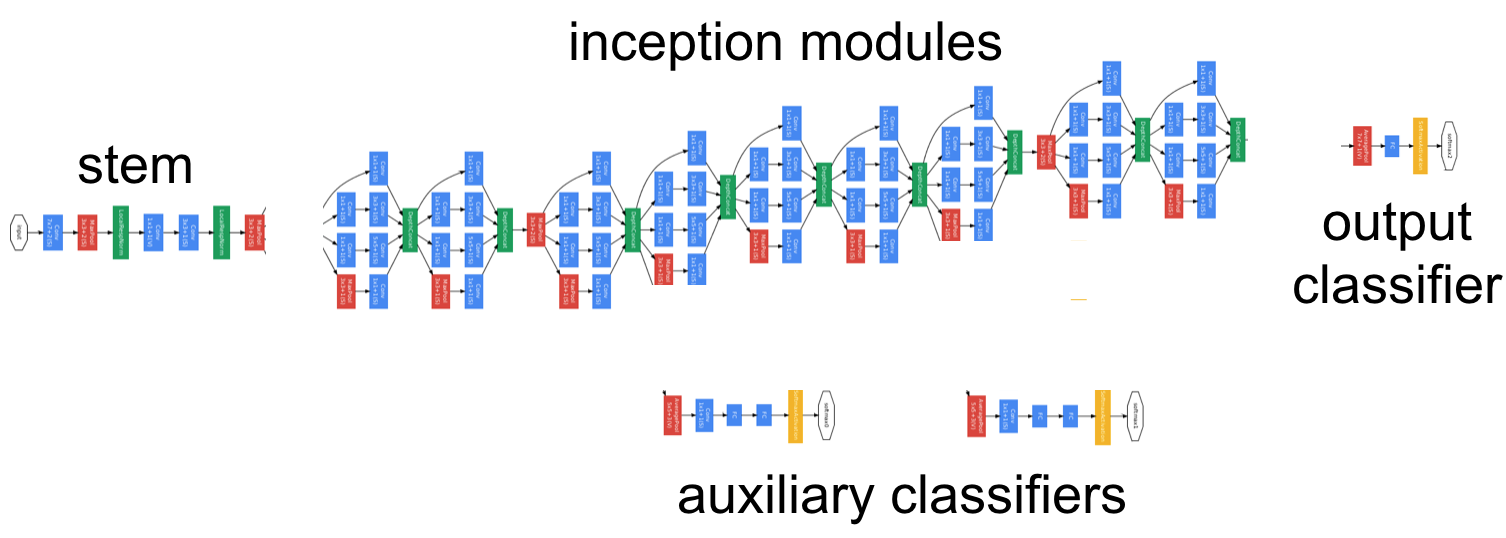
\includegraphics[width=\linewidth]{inception.png}
    \imageright{Joe Marino}
\end{figure}
\end{frame}

\begin{frame}
\frametitle{Inception}

\begin{columns}
    \begin{column}{0.38\textwidth}
        \begin{itemize}
            \item Winner of ILSVRC 2014
            \item Repeating same kernels
            \item \textbf{Idea:} repeating Inception module
            \item Core concept
            \begin{itemize}
                \item Cheap non-linearities ($1\times 1$ convolution)
                \item Different resolution scales
            \end{itemize}
        \end{itemize}
    \end{column}
    \begin{column}{0.58\textwidth}
        \begin{figure}
            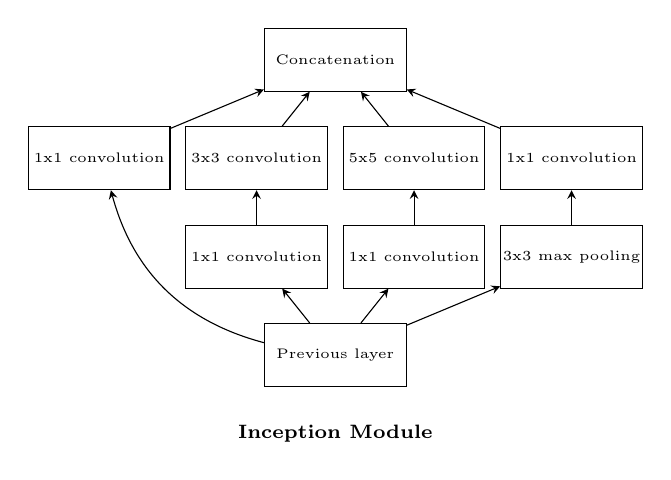
\begin{tikzpicture}
                \node[draw, rectangle, align=center, minimum width=1.8cm, minimum height=0.8cm, inner sep=0cm] (concat) at (0, 1) {\tiny Concatenation};
            
                \node[draw, rectangle, align=center, minimum width=1.8cm, minimum height=0.8cm, inner sep=0cm] (left 2) at (-3, -0.25) {\tiny 1x1 convolution};
                \node[draw, rectangle, align=center, minimum width=1.8cm, minimum height=0.8cm, inner sep=0cm] (mid left 2) at (-1, -0.25) {\tiny 3x3 convolution};
                \node[draw, rectangle, align=center, minimum width=1.8cm, minimum height=0.8cm, inner sep=0cm] (mid right 2) at (1, -0.25) {\tiny 5x5 convolution};
                \node[draw, rectangle, align=center, minimum width=1.8cm, minimum height=0.8cm, inner sep=0cm] (right 2) at (3, -0.25) {\tiny 1x1 convolution};
                
                \node[draw, rectangle, align=center, minimum width=1.8cm, minimum height=0.8cm, inner sep=0cm] (mid left 1) at (-1, -1.5) {\tiny 1x1 convolution};
                \node[draw, rectangle, align=center, minimum width=1.8cm, minimum height=0.8cm, inner sep=0cm] (mid right 1) at (1, -1.5) {\tiny 1x1 convolution};
                \node[draw, rectangle, align=center, minimum width=1.8cm, minimum height=0.8cm, inner sep=0cm] (right 1) at (3, -1.5) {\tiny 3x3 max pooling};
                
                \node[draw, rectangle, align=center, minimum width=1.8cm, minimum height=0.8cm, inner sep=0cm] (previous) at (0, -2.75) {\tiny Previous layer};
                
                \draw[->, >=stealth] (left 2)--(concat);
                \draw[->, >=stealth] (mid left 2)--(concat);
                \draw[->, >=stealth] (mid right 2)--(concat);
                \draw[->, >=stealth] (right 2)--(concat);
                
                \draw[->, >=stealth] (mid left 1)--(mid left 2);
                \draw[->, >=stealth] (mid right 1)--(mid right 2);
                \draw[->, >=stealth] (right 1)--(right 2);
                
                \path[->, >=stealth] (previous) edge [bend left] (left 2);
                \draw[->, >=stealth] (previous)--(mid left 1);
                \draw[->, >=stealth] (previous)--(mid right 1);
                \draw[->, >=stealth] (previous)--(right 1);
                
                \node at (0, -3.75) {\scriptsize\textbf{Inception Module}};
            \end{tikzpicture}
        \end{figure}
    \end{column}
\end{columns}
\end{frame}

\begin{frame}
\frametitle{ResNet}

\begin{figure}
    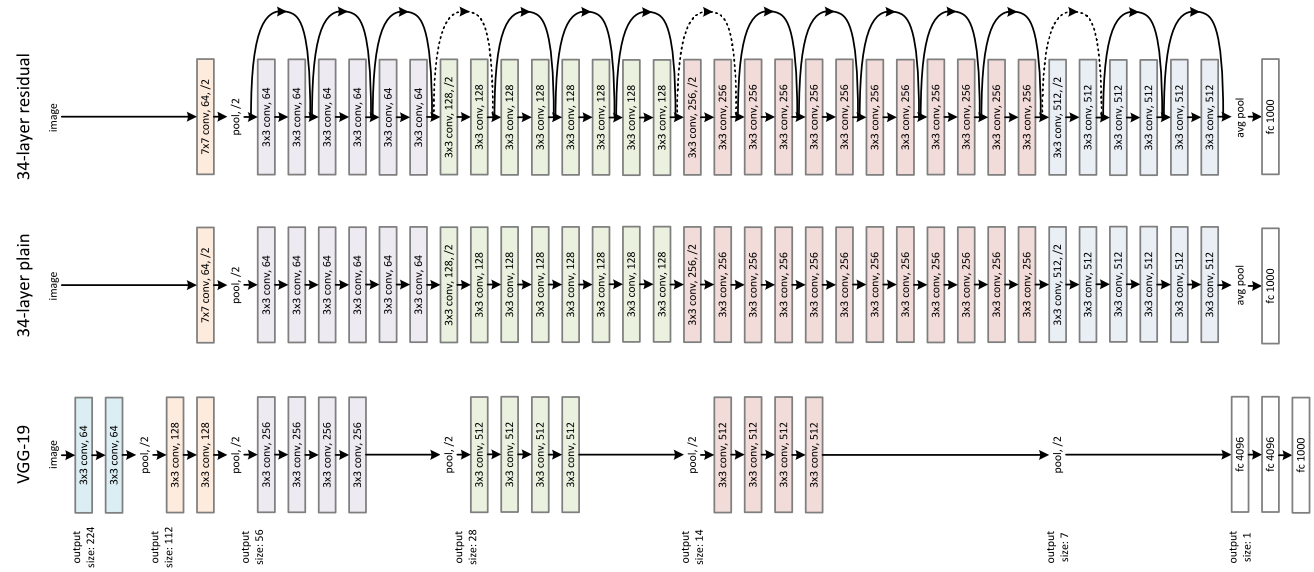
\includegraphics[width=\linewidth]{resnet.jpg}
    \imageright{Medium}
\end{figure}
\end{frame}


\begin{frame}
\frametitle{Residual Unit}

\begin{columns}
    \begin{column}{0.48\textwidth}
        \begin{itemize}
            \item Winner of ILSVRC 2015
            \item Ultra deep network (152 layers)
            \item \textbf{Idea:} nested mini networks
            \begin{itemize}
                \item Learn residuals and add to input
                \item Unused units do nothing
            \end{itemize}
            \item First time, humans have been surpassed
        \end{itemize}
    \end{column}
    \begin{column}{0.48\textwidth}
        \begin{figure}
            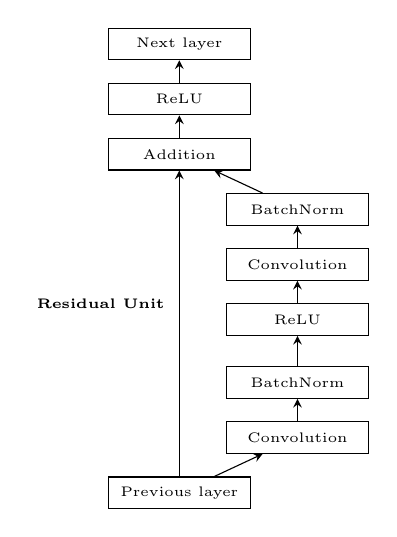
\begin{tikzpicture}
                \node[draw, rectangle, align=center, minimum width=1.8cm, minimum height=0.4cm, inner sep=0cm] (next layer) at (0, 2.7) {\tiny Next layer};
                \node[draw, rectangle, align=center, minimum width=1.8cm, minimum height=0.4cm, inner sep=0cm] (relu out) at (0, 2.0) {\tiny ReLU};
                \node[draw, rectangle, align=center, minimum width=1.8cm, minimum height=0.4cm, inner sep=0cm] (addition) at (0, 1.3) {\tiny Addition};
                
                \node[draw, rectangle, align=center, minimum width=1.8cm, minimum height=0.4cm, inner sep=0cm] (5) at (1.5, 0.6) {\tiny BatchNorm};
                \node[draw, rectangle, align=center, minimum width=1.8cm, minimum height=0.4cm, inner sep=0cm] (4) at (1.5, -0.1) {\tiny Convolution};
                \node[draw, rectangle, align=center, minimum width=1.8cm, minimum height=0.4cm, inner sep=0cm] (3) at (1.5, -0.8) {\tiny ReLU};
                \node[draw, rectangle, align=center, minimum width=1.8cm, minimum height=0.4cm, inner sep=0cm] (2) at (1.5, -1.6) {\tiny BatchNorm};
                \node[draw, rectangle, align=center, minimum width=1.8cm, minimum height=0.4cm, inner sep=0cm] (1) at (1.5, -2.3) {\tiny Convolution};
                
                \node[draw, rectangle, align=center, minimum width=1.8cm, minimum height=0.4cm, inner sep=0cm] (previous) at (0, -3) {\tiny Previous layer};
                
                \draw[->, >=stealth] (previous)--(addition);
                \draw[->, >=stealth] (previous)--(1);
                \draw[->, >=stealth] (1)--(2);
                \draw[->, >=stealth] (2)--(3);
                \draw[->, >=stealth] (3)--(4);
                \draw[->, >=stealth] (4)--(5);
                \draw[->, >=stealth] (5)--(addition);
                \draw[->, >=stealth] (addition)--(relu out);
                \draw[->, >=stealth] (relu out)--(next layer);
                
                \node at (-1.0, -0.6) {\tiny\textbf{Residual Unit}};
            \end{tikzpicture}
        \end{figure}
    \end{column}
\end{columns}
\end{frame}

\begin{frame}
\frametitle{Deep Learning Issues}

\begin{itemize}
    \item \textbf{GPU memory size:} forward and backward passes need to be stored\\
    network parameters need to be stored\\
    Counter by decreasing batch sizes, use multipe GPUs
    \item \textbf{Vanishing and shattered gradients:} gradients become too small or noise the deeper you stack the network\\
    \item \textbf{Debugging:} almost impossible to understand what each components does\\
    Some tools available: Influence functions, layer output investigation
\end{itemize}
\end{frame}

\begin{frame}[fragile]
\frametitle{CNNs in Keras}

\begin{lstlisting}[language=Python]
from keras.models import Sequential
from keras.layers import BatchNormalization, Conv2D,
                         Dense, MaxPooling2D
from keras.regularizers import l2

# Convolutional neural network
w, h, c = 128, 128, 1 # width, height, channels
model = Sequential()
model.add(Conv2D(16, (5, 5), padding="same", input_shape=(w, h, c))}
model.add(MaxPooling2D((2, 2), strides=(1, 1))}
model.add(BatchNormalization())}
model.add(Dense(128)
model.add(Dense(classes, activation='softmax'))

# Model compilation
model.compile(loss="categorical_crossentropy", optimizer="sgd")
\end{lstlisting}

\end{frame}

\begin{frame}[fragile]
\frametitle{Keras Functional API}

\begin{lstlisting}[language=Python]
from keras.models import Model
from keras.layers import Dense, Input

features = 20
data = Input(shape=(features,))

# layers can be connected by calling the previous layer
layer_1 = Dense(64)(data)
layer_2 = Dense(64)(layer_1)
predict = Dense(10, activation="softmax")(layer_2)

# the model must be created manually
model = Model(inputs=[data], outputs=[predict])
\end{lstlisting}

\end{frame}

\subsection{Exercise: MNIST CNN}
\label{subsec:cnn-exercise}

\begin{frame}
\frametitle{Exercise: CNN MNIST Image Classification}

\begin{figure}
    \centering
    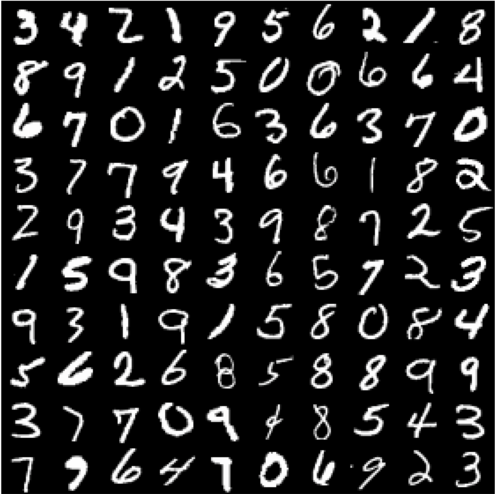
\includegraphics[width=0.4\linewidth]{mnist.png}
\end{figure}
\end{frame}

\section{Regression}
\label{sec:regression}

\begin{frame}
\frametitle{Abalone Dataset}

\begin{columns}
    \begin{column}{0.48\textwidth}
        \begin{itemize}
            \item Collected by the University of Tasmania, Australia
            \item \textbf{Abalones are ``sea snails''}
            \item 4177 instances, each 9 features
            \item Prediction task
            \begin{itemize}
                \item Regress age ($rings + 1.5$) of abalone
                \item Requires manual preprocessing
                \item Reduce microscopy cost and labor
            \end{itemize}
        \end{itemize}
    \end{column}
    \begin{column}{0.48\textwidth}
        \begin{figure}
            \centering
            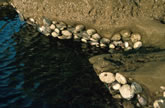
\includegraphics[width=0.8\linewidth]{abalone2.jpg}
            \imageright{UCI Machine Learning Repository}
        \end{figure}
    \end{column}
\end{columns}
\end{frame}

\subsection{Exercise: Abalone}
\label{subsec:regression-exercise}

\begin{frame}
    \frametitle{Exercise: Abalone Age Regression Analysis}
    \begin{figure}
        \centering
        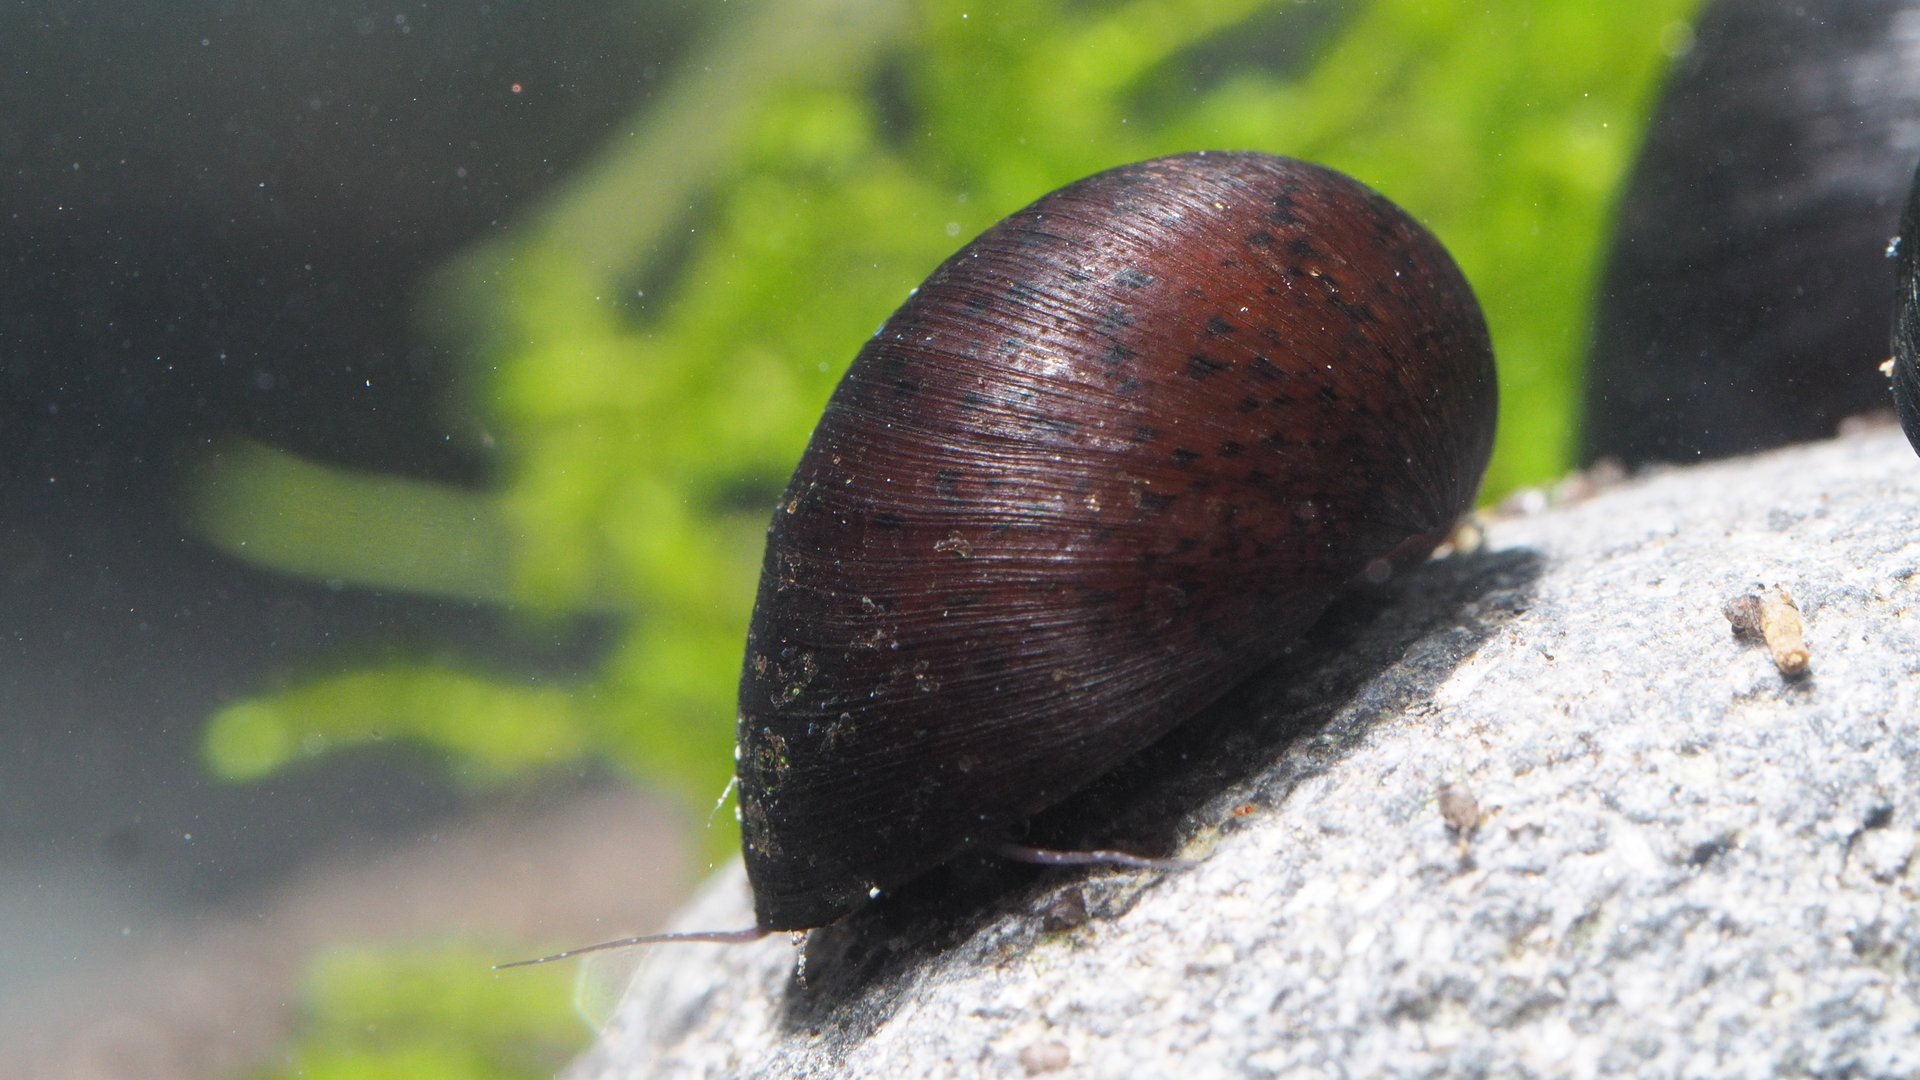
\includegraphics[width=0.7\linewidth]{abalone.jpg}
        \imageright{Garnelaxia}
    \end{figure}
\end{frame}

\section{Summary}
\label{sec:summary}

\begin{frame}
\frametitle{Summary}

\begin{itemize}
    \item \textbf{Supervised machine learning}
    \begin{itemize}
        \item Logistic regression
        \item Fully-connected neural networks (\textbf{FNN})
        \item Convolution neural networks (\textbf{CNN})
    \end{itemize}
    \item Network components
    \begin{itemize}
        \item Activation functions
        \item Regularization
        \item Optimizers
    \end{itemize}
    \item Application scenarios, \textbf{regression} and \textbf{classification}
\end{itemize}
\end{frame}

\begin{frame}
\frametitle{What's more?}

\begin{itemize}
    \item \textbf{Data augmentation:} artificial data increase through rotation, scaling,\\ translation, etc. to better abstract patterns and increase data set size
    \item \textbf{Embedding:} lower-dimensional representation of (sparse) input data
    \item \textbf{Capsule Networks:} hierarchy and translation-aware neural networks
    \item \textbf{Recurrent Neural Networks (RNN):} sequence-learning neural networks,\\ e.g natural language processing and time series analysis
    \item \textbf{Attention:} learning ``where to look'', e.g. for natural language translation
\end{itemize}
\end{frame}

\begin{frame}
\frametitle{Acknowledgment}

\begin{columns}
    \begin{column}{0.48\textwidth}
        \begin{itemize}
            \item \textbf{Eileen Kühn}
            \begin{itemize}
                \item GridKa School organization
                \item Paperwork
            \end{itemize}
            \item \textbf{Oskar Taubert}
            \begin{itemize}
                \item Assignment preparation
                \item Exercise supervision
            \end{itemize}
            \item \textbf{Andreas Herten}
            \begin{itemize}
                \item Access to JURON
                \item Technical support
            \end{itemize}
        \end{itemize}
    \end{column}

    \begin{column}{0.48\textwidth}
        \begin{figure}
            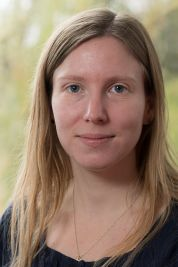
\includegraphics[width=0.25\linewidth]{eileen.jpg}\quad 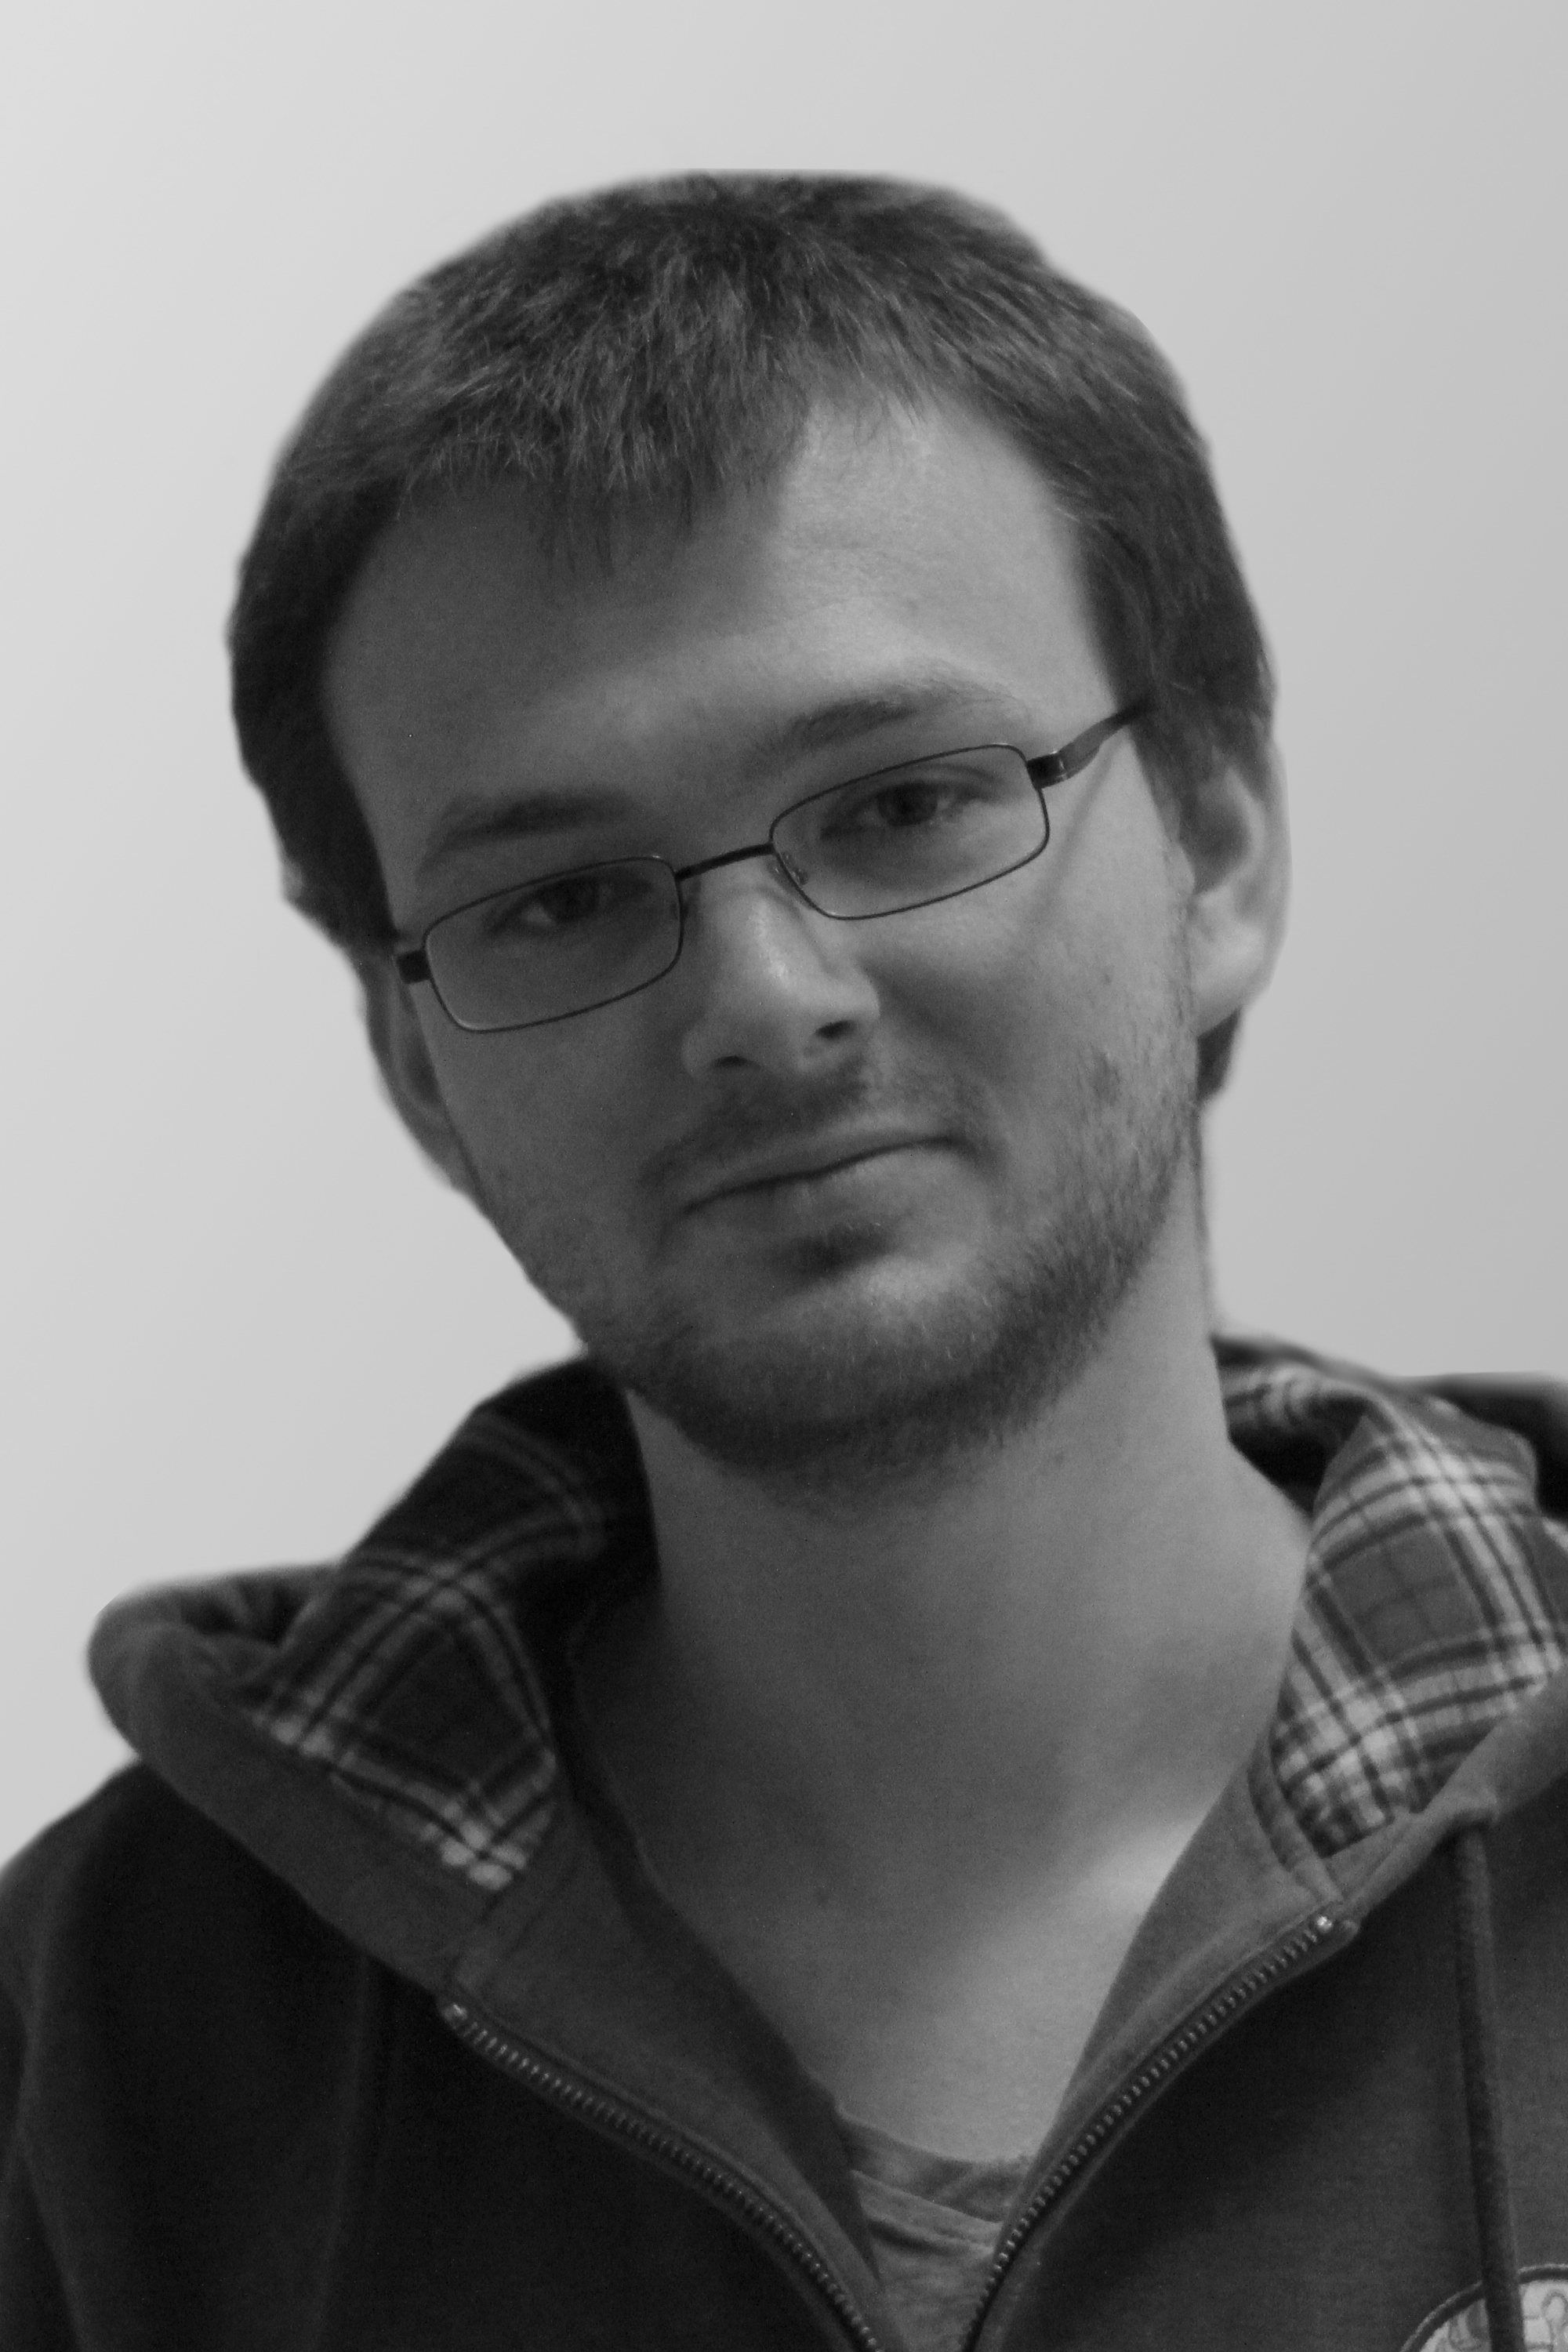
\includegraphics[width=0.25\linewidth]{oskar.jpg} \\\medskip
            
            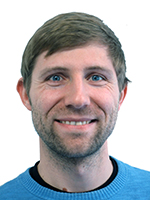
\includegraphics[width=0.25\linewidth]{andreas.jpg}\quad 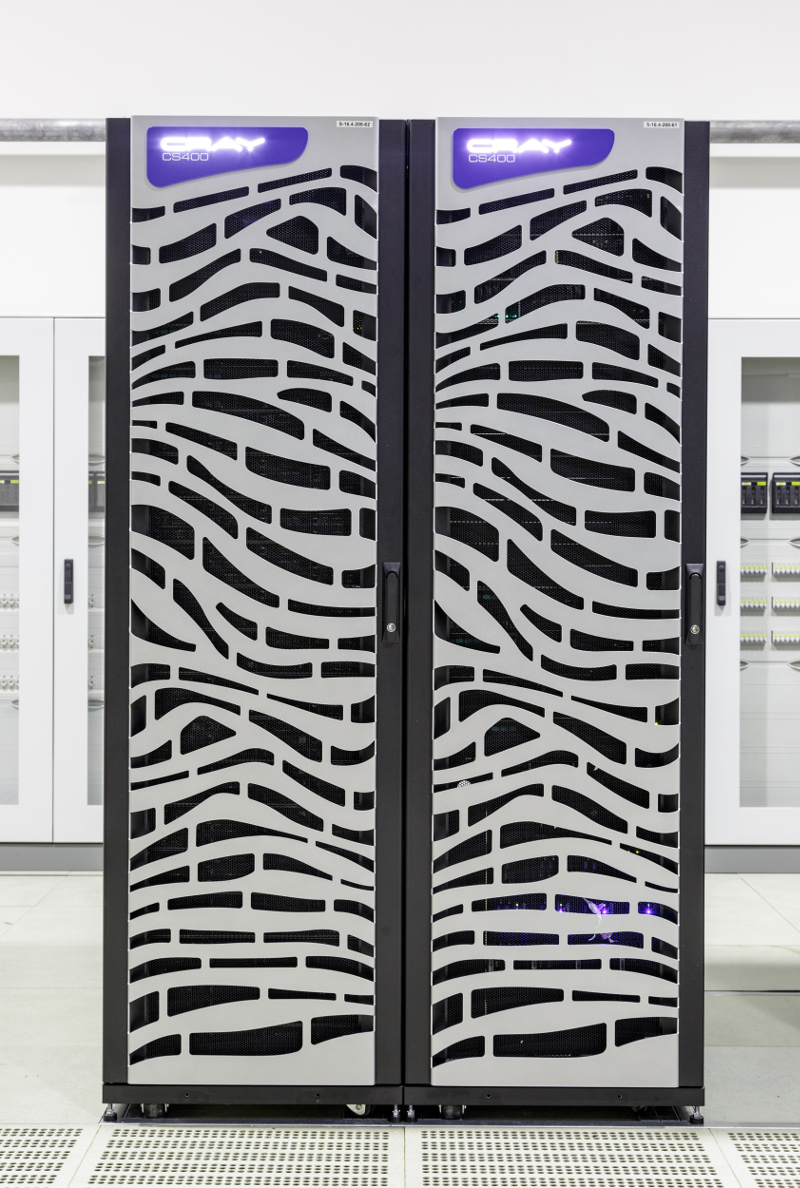
\includegraphics[width=0.25\linewidth]{juron.jpg} \\
        \end{figure}
    \end{column}
\end{columns}
\end{frame}

\section{Discussion}
\label{sec:discussion}

\end{document}
